\documentclass[10pt,aspectratio=43]{beamer}

\usepackage{graphicx}
\usepackage{tikz}
\usepackage{xcolor}
\usepackage{caption}
\usepackage{subcaption}
\usepackage{bm}
\usetikzlibrary{calc} 
\usepackage{hyperref}
\hypersetup{
    colorlinks=true,
    linkcolor=blue,
    urlcolor=red
}
\usepackage{fontawesome5}
\usepackage{ulem}

\usetheme{MyStyle}   % loads beamerthemeMyStyle.sty
\setlength{\columnsep}{0pt}


%%%%%%%%%%%%%%%%%%%%%%%%%%%%%%%%%%%%%%%%%%
%%%%%%%%%%%%%%%%%%%%%%%%%%%%%%%%%%%%%%%%%%
%%%%%%%%%%%%%%%%%%%%%%%%%%%%%%%%%%%%%%%%%%

\title{AHDC wire swaps - results}
\newcommand{\eventname}{ALERT meeting}
\author{Felix Touchte Codjo}
\institute{IJCLab}
\date{\today}


\begin{document}

\begin{frame}[plain] % remove header, footer, barre de navigation
\titlepage
\end{frame}

%\begin{frame}{Outline}
%\tableofcontents
%\end{frame}

%\section{Intro}
\section{Updates}

\begin{frame}{Results - wire swaps}
    \begin{itemize}
        \item Summary of wire swaps
    \end{itemize}

    \centering
    \vspace{0.2cm}

    \begin{tabular}{cccc}
        1. & L21W18 & $\longleftrightarrow$ & L21W19 \\
        2. & L22W20 & $\longleftrightarrow$ & L22W22 \\
        3. & L22W42 & $\longleftrightarrow$ & L22W43 \\
        4. & L31W68 & $\longleftrightarrow$ & L32W68 \\
    \end{tabular}

    \vspace{0.2cm}
    \begin{itemize}
        \item Comments
        
            \begin{itemize}
                \item The first 3 swaps appear when we plot the wire occupancy versus the electron phi
                \item The last one appear when we look at the residuals distributions
                \item Others residual distributions had a bad shape, but they all had a bad $t_0$. Their distributions became good when we set them a reasonable value of $t_0$.
            \end{itemize}
    \end{itemize}
    
\end{frame}

\begin{frame}{Results - wire swaps}
    \begin{itemize}
        \item Illustration : Wire versus phi (old translation table)
    \end{itemize}

    \centering
    \vspace{0.2cm}

    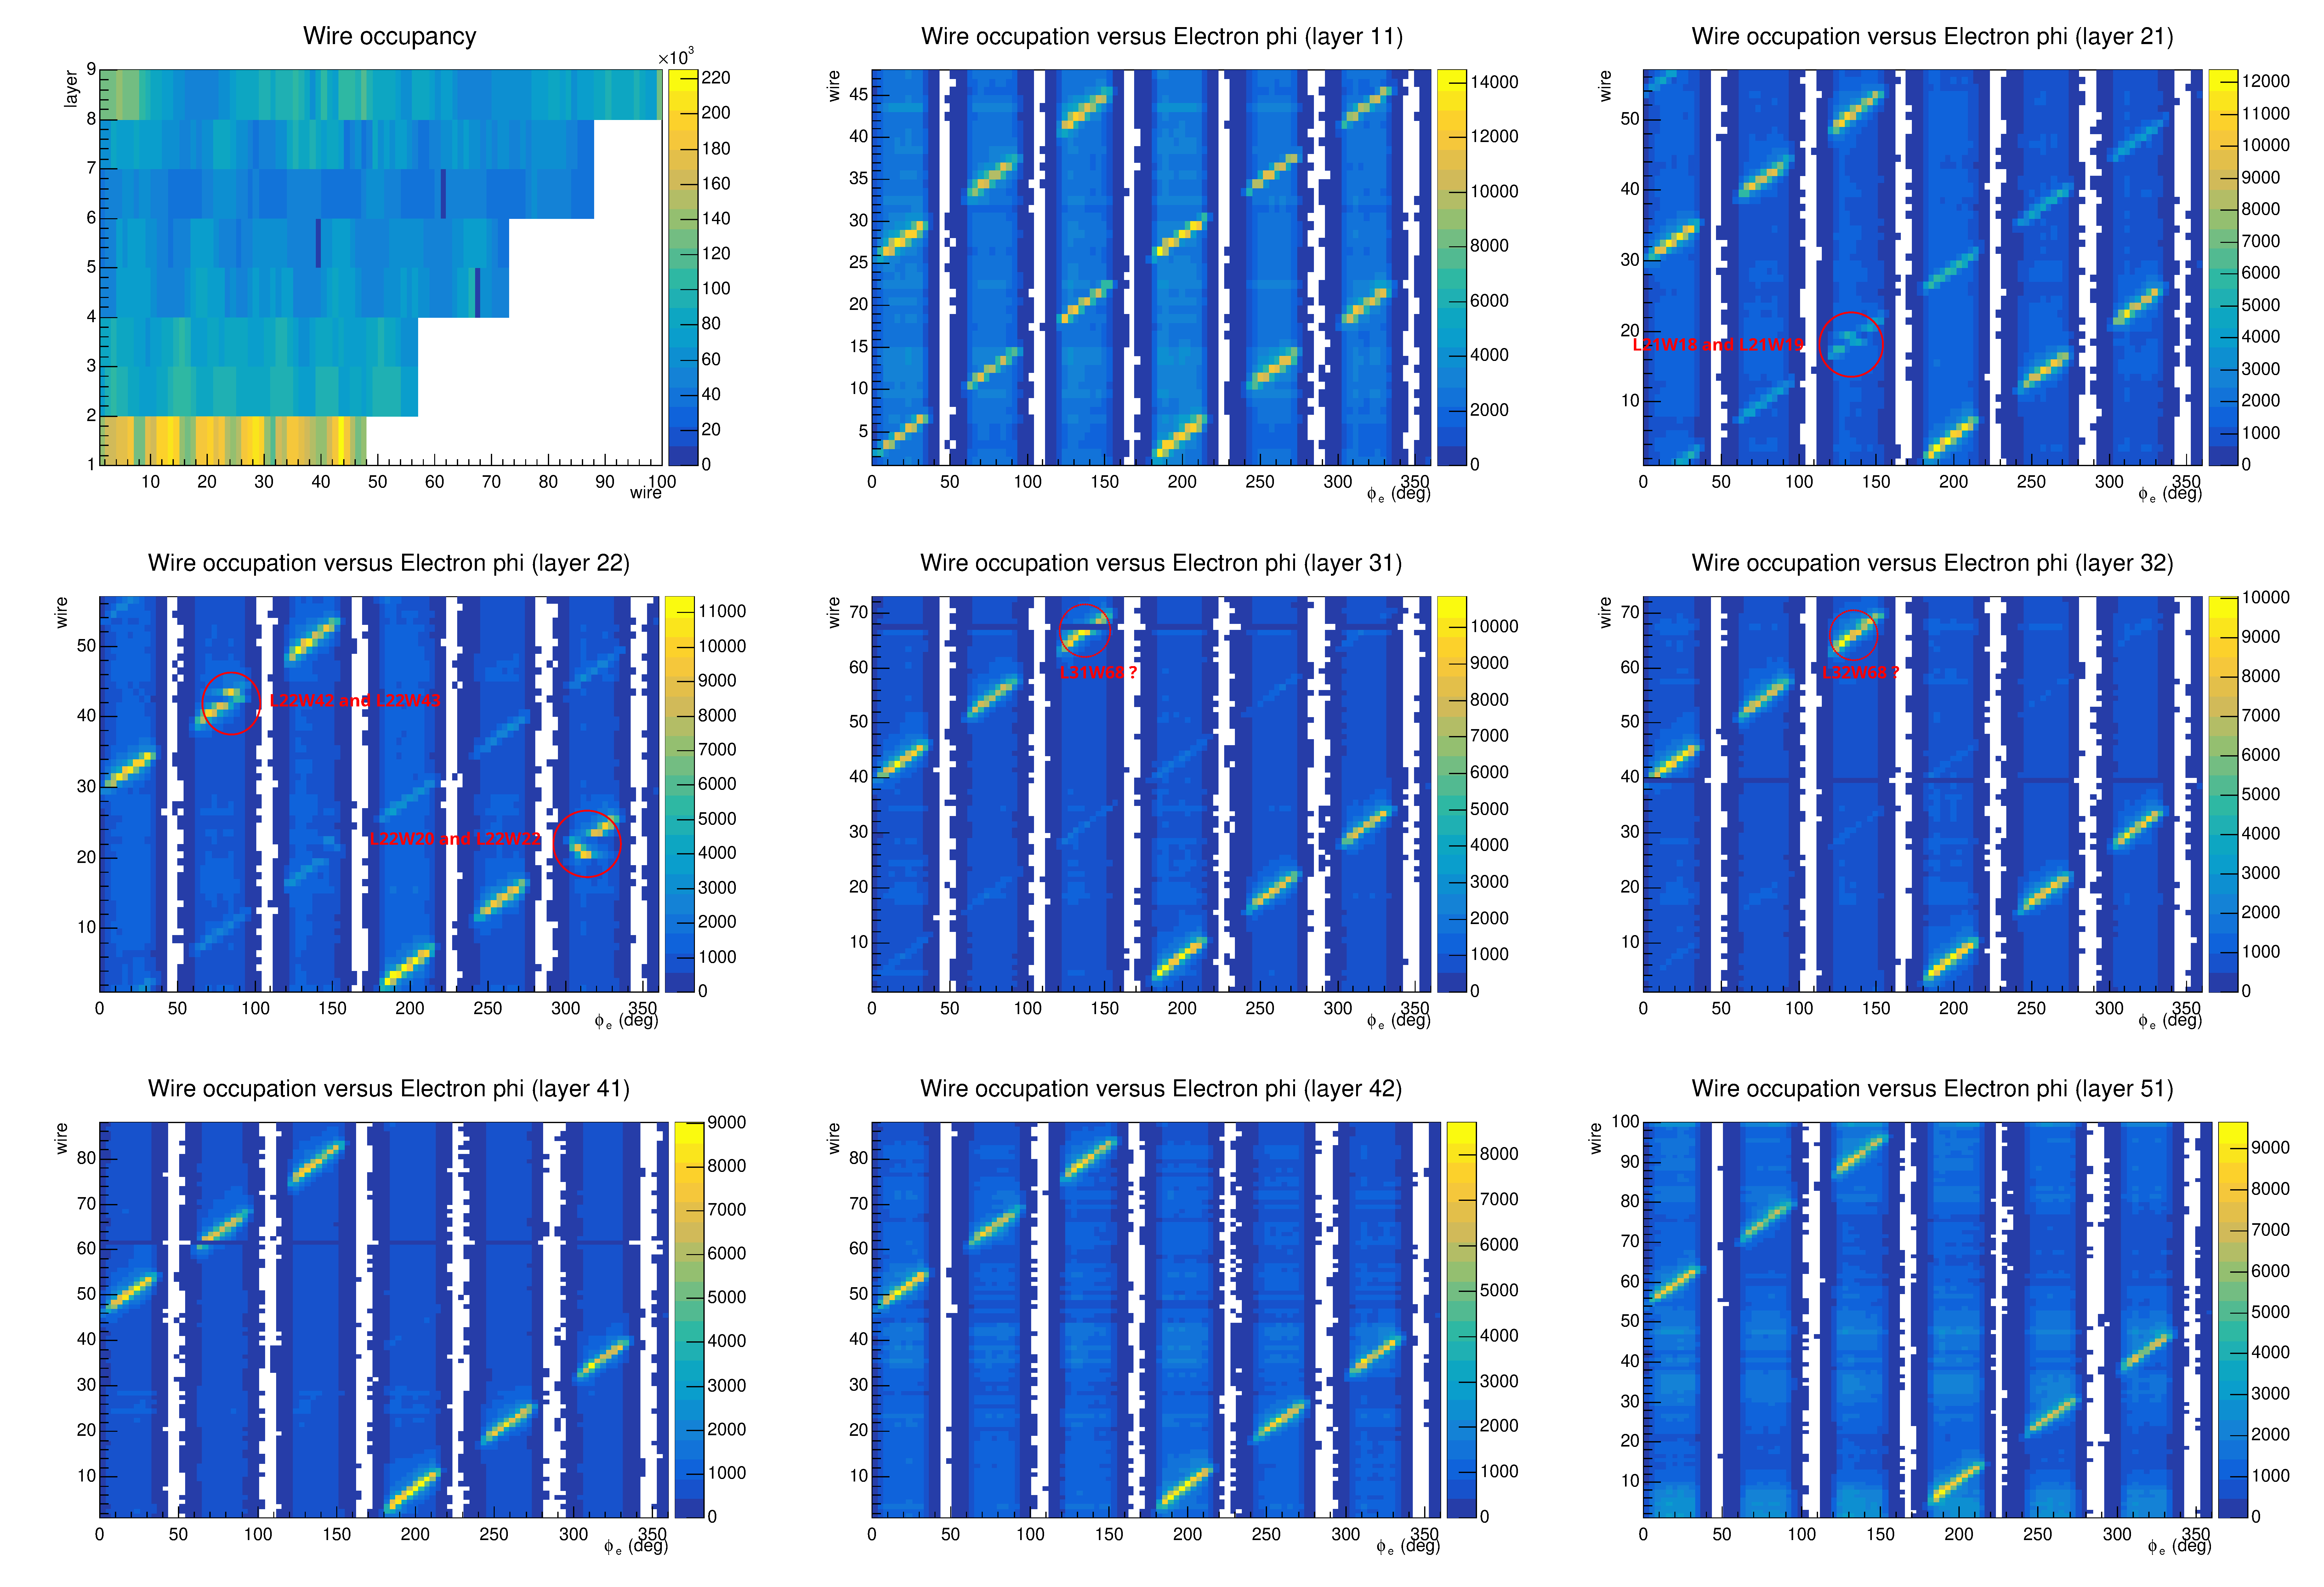
\includegraphics[width=0.8\linewidth]{figures/wire_versus_phi_old_translation_table_annotated.pdf}

\end{frame}

\begin{frame}{Results - wire swaps}
    \begin{itemize}
        \item Illustration :  Wire versus phi (new translation table)
    \end{itemize}

    \centering
    \vspace{0.2cm}

    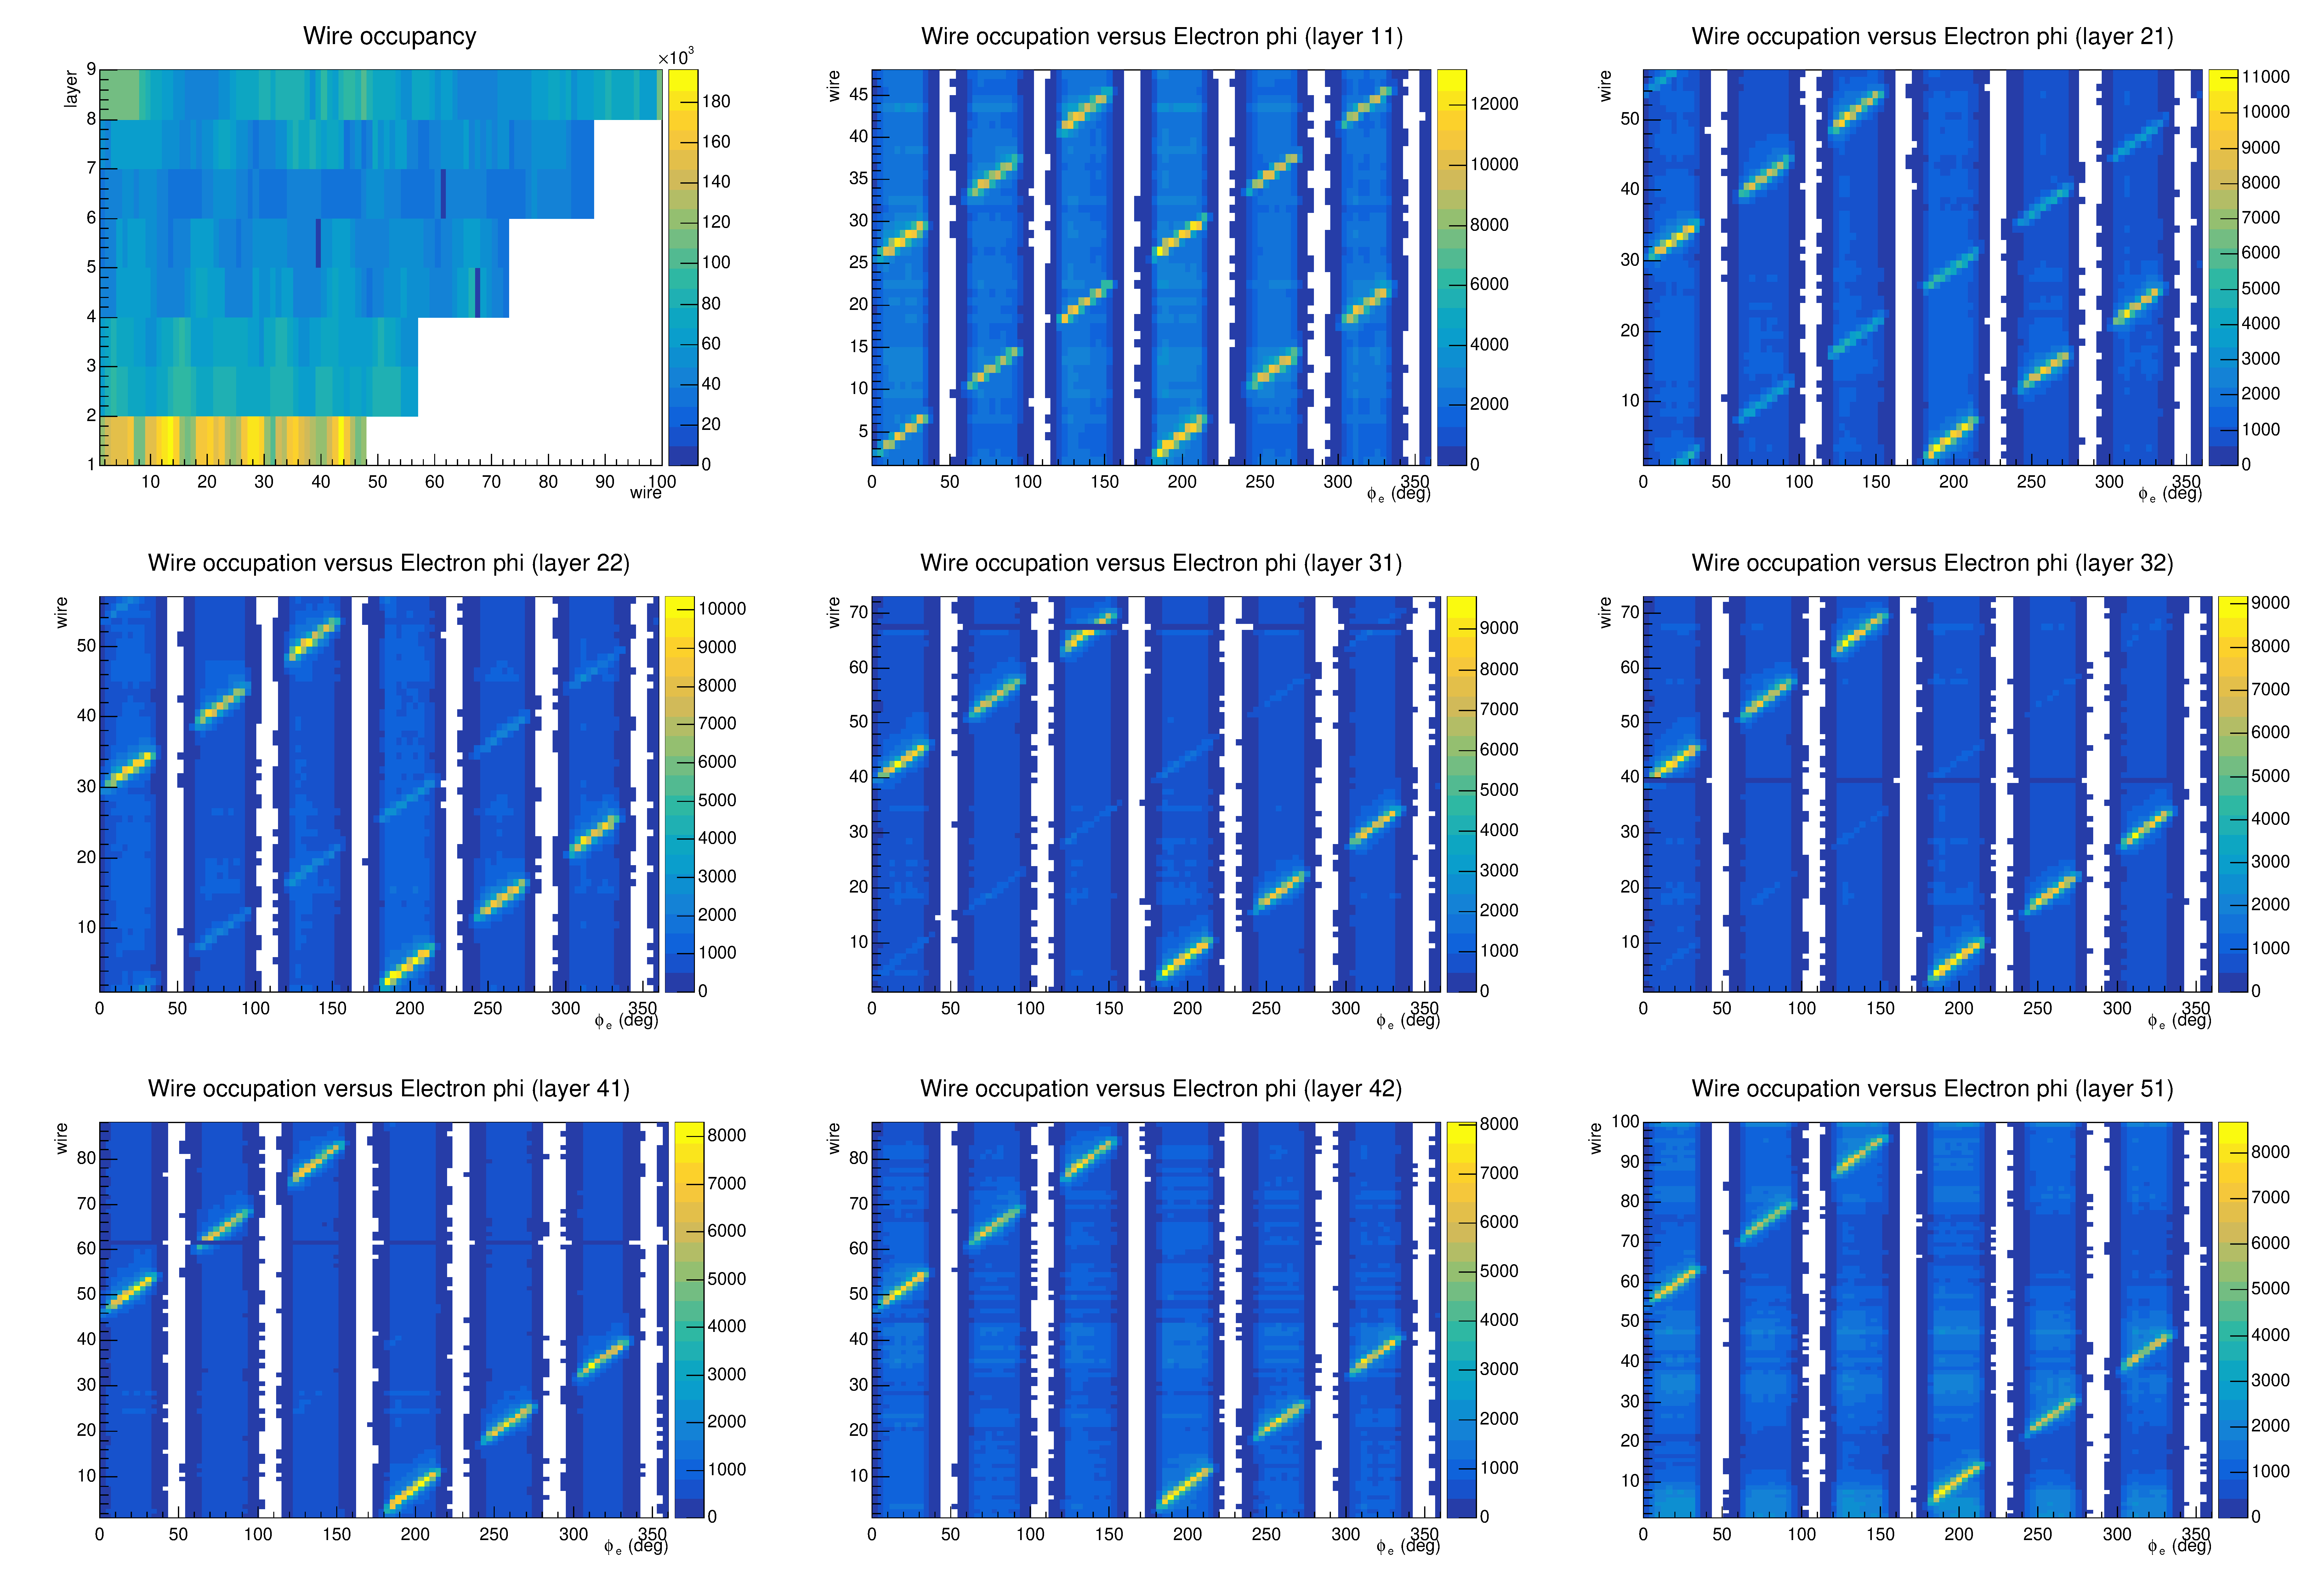
\includegraphics[width=0.8\linewidth]{figures/wire_versus_phi_new_translation_table.pdf}

\end{frame}


\begin{frame}{Results - wire swaps}
    \begin{itemize}
        \item Illustration :  Residual distributions before and after the swaps
    \end{itemize}

    \centering
    \vspace{0.1cm}

    
    \begin{tabular}{cc|cc}
        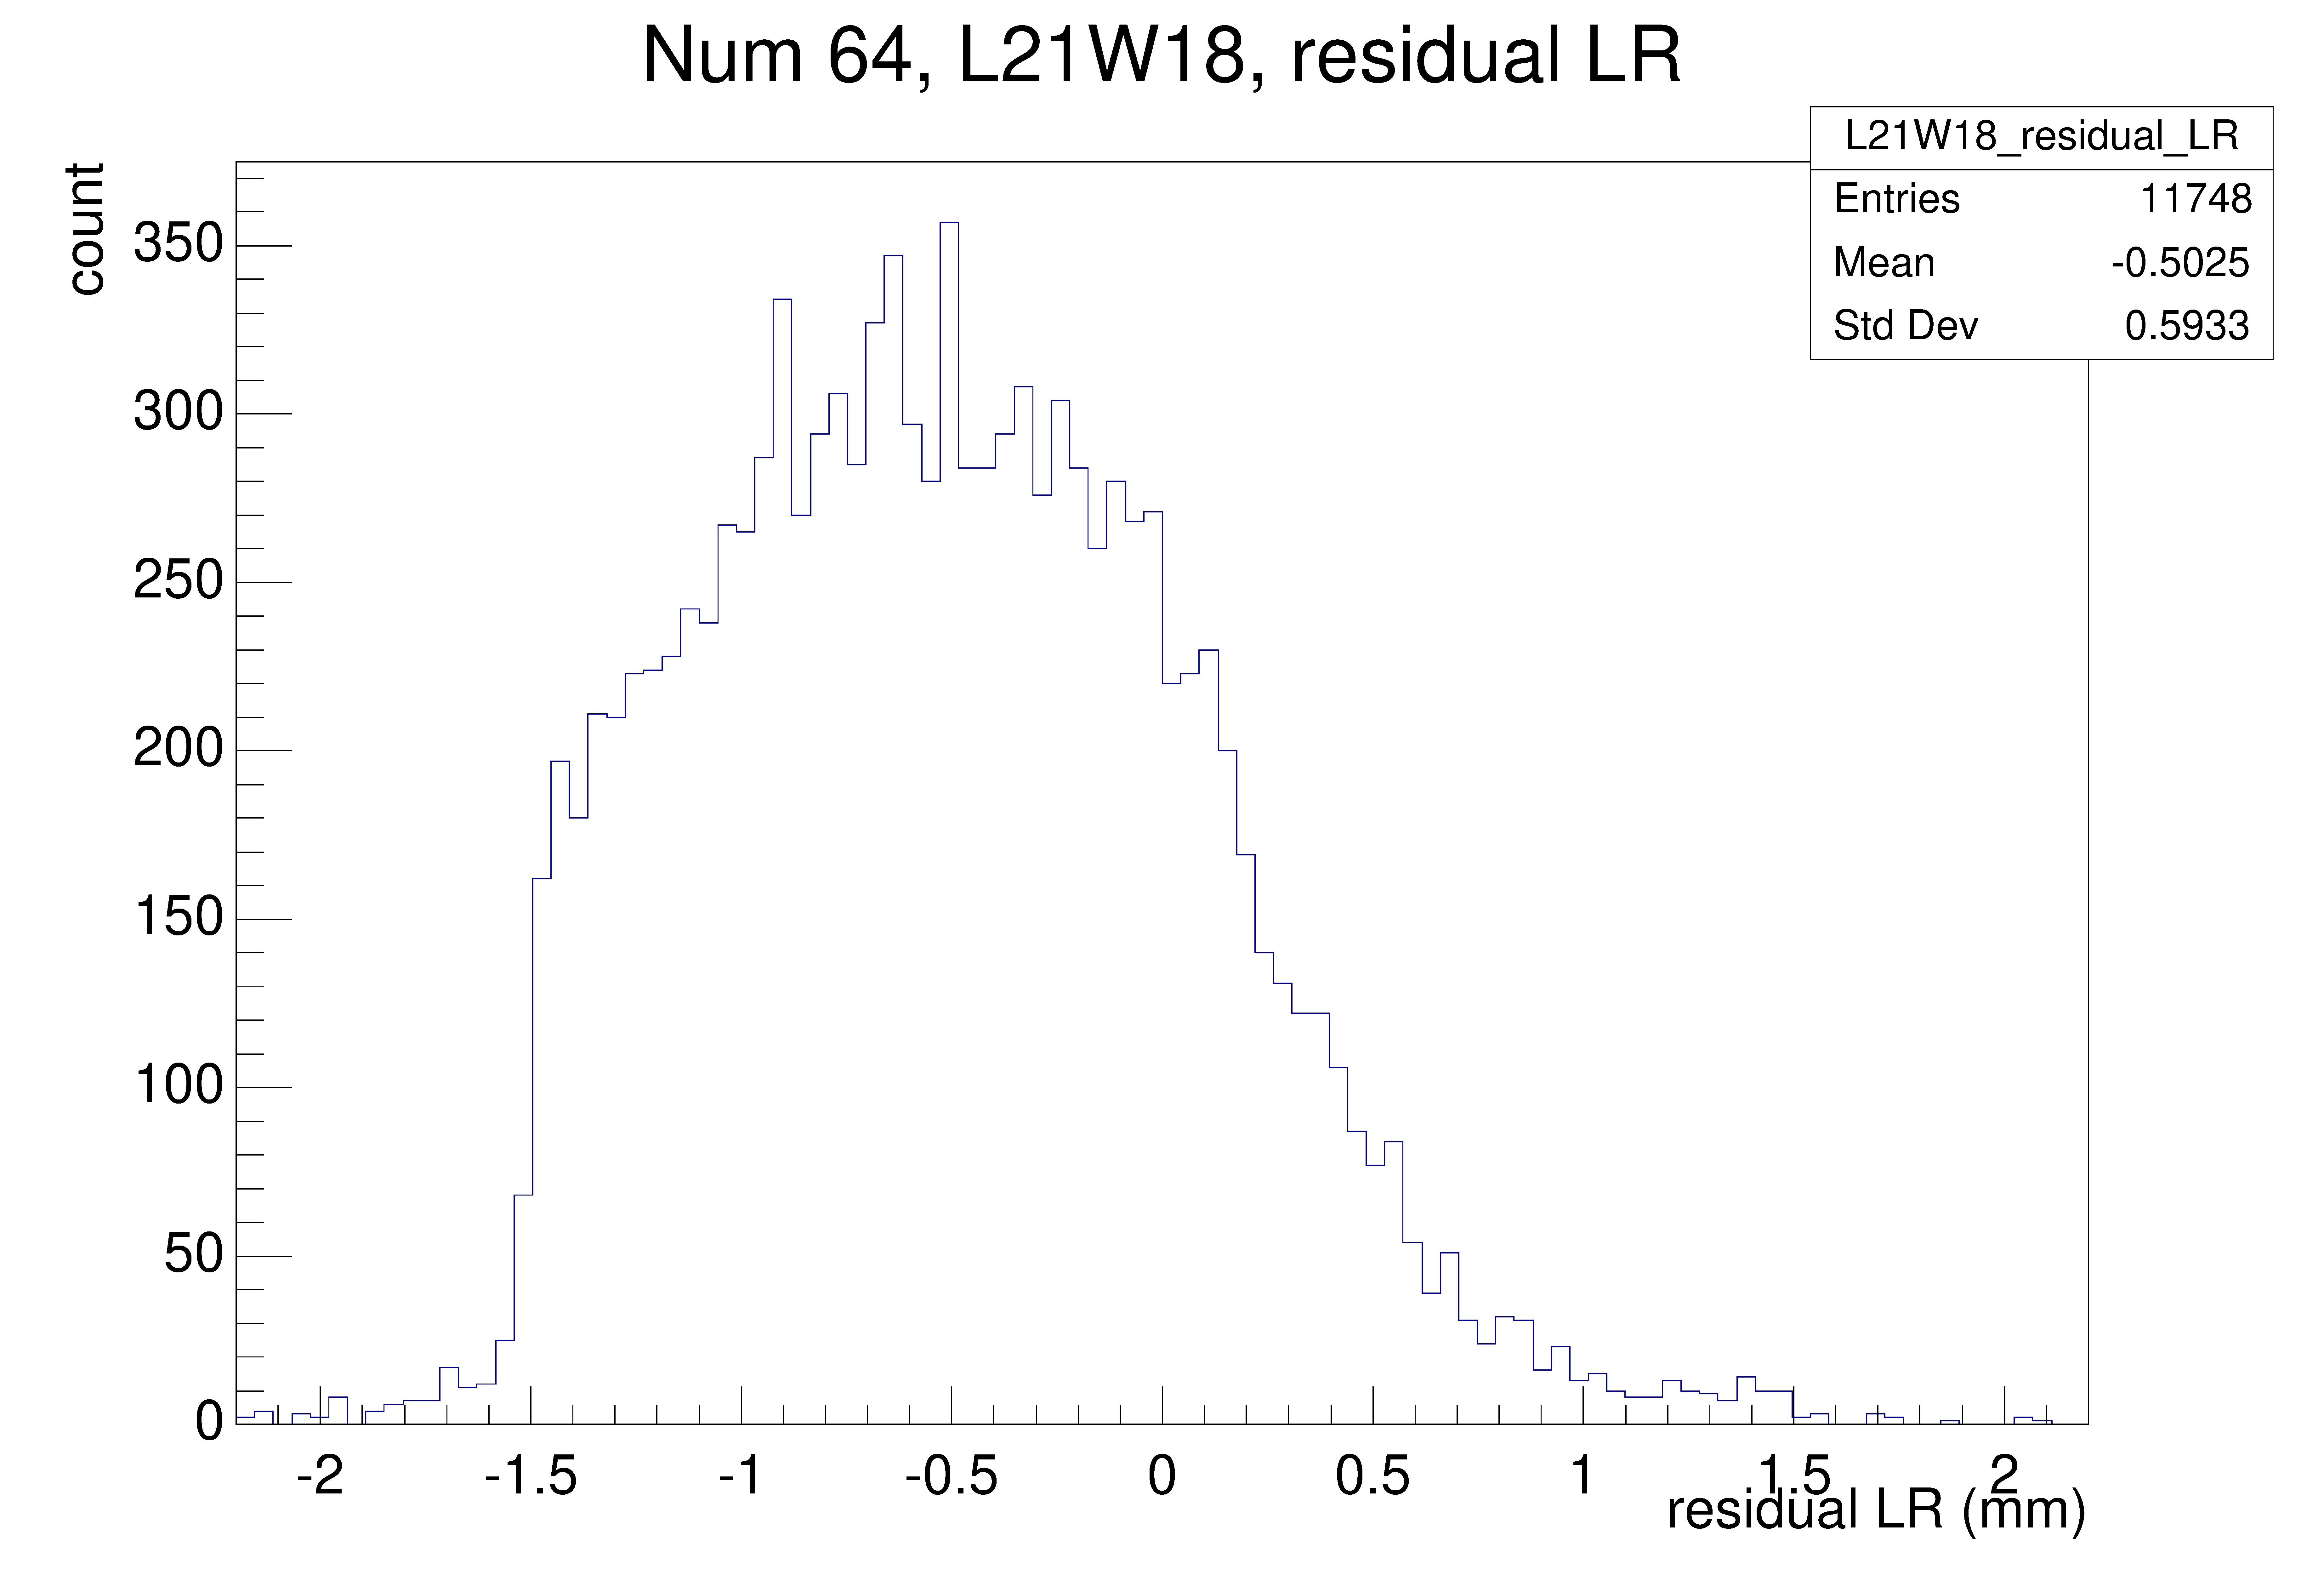
\includegraphics[width=0.20\linewidth]{figures/L21W18_old_tt.pdf} & 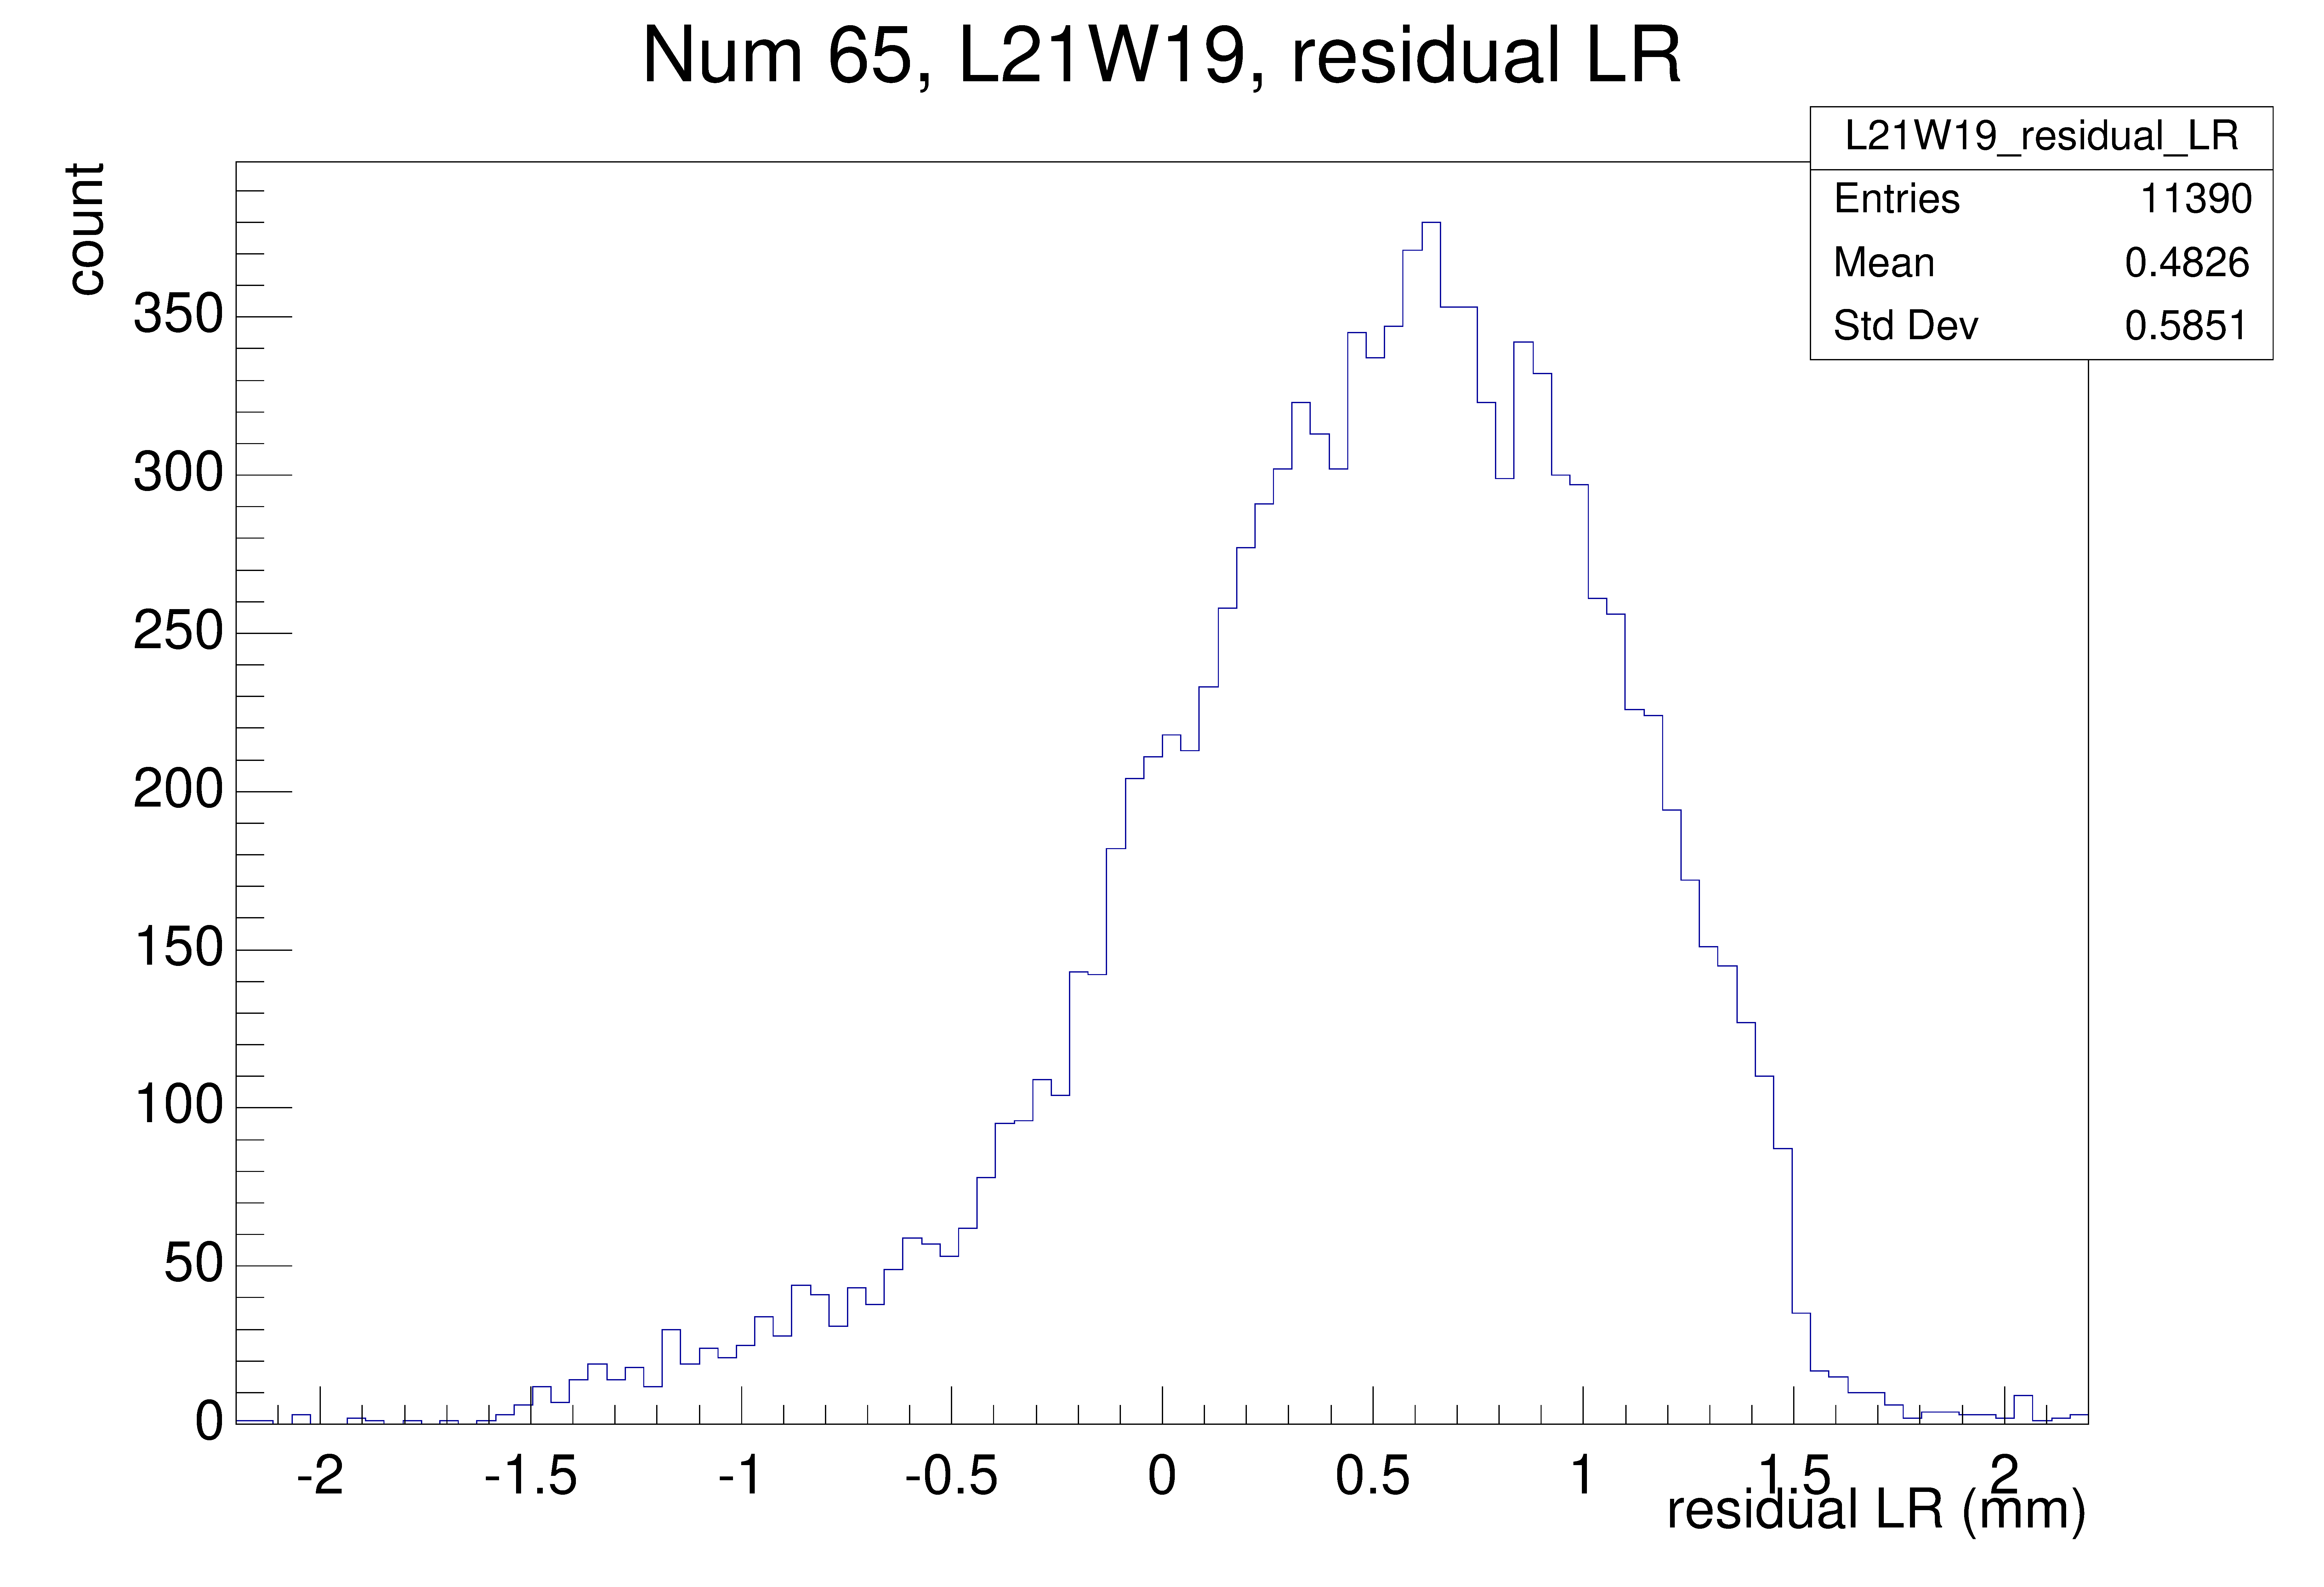
\includegraphics[width=0.20\linewidth]{figures/L21W19_old_tt.pdf} & 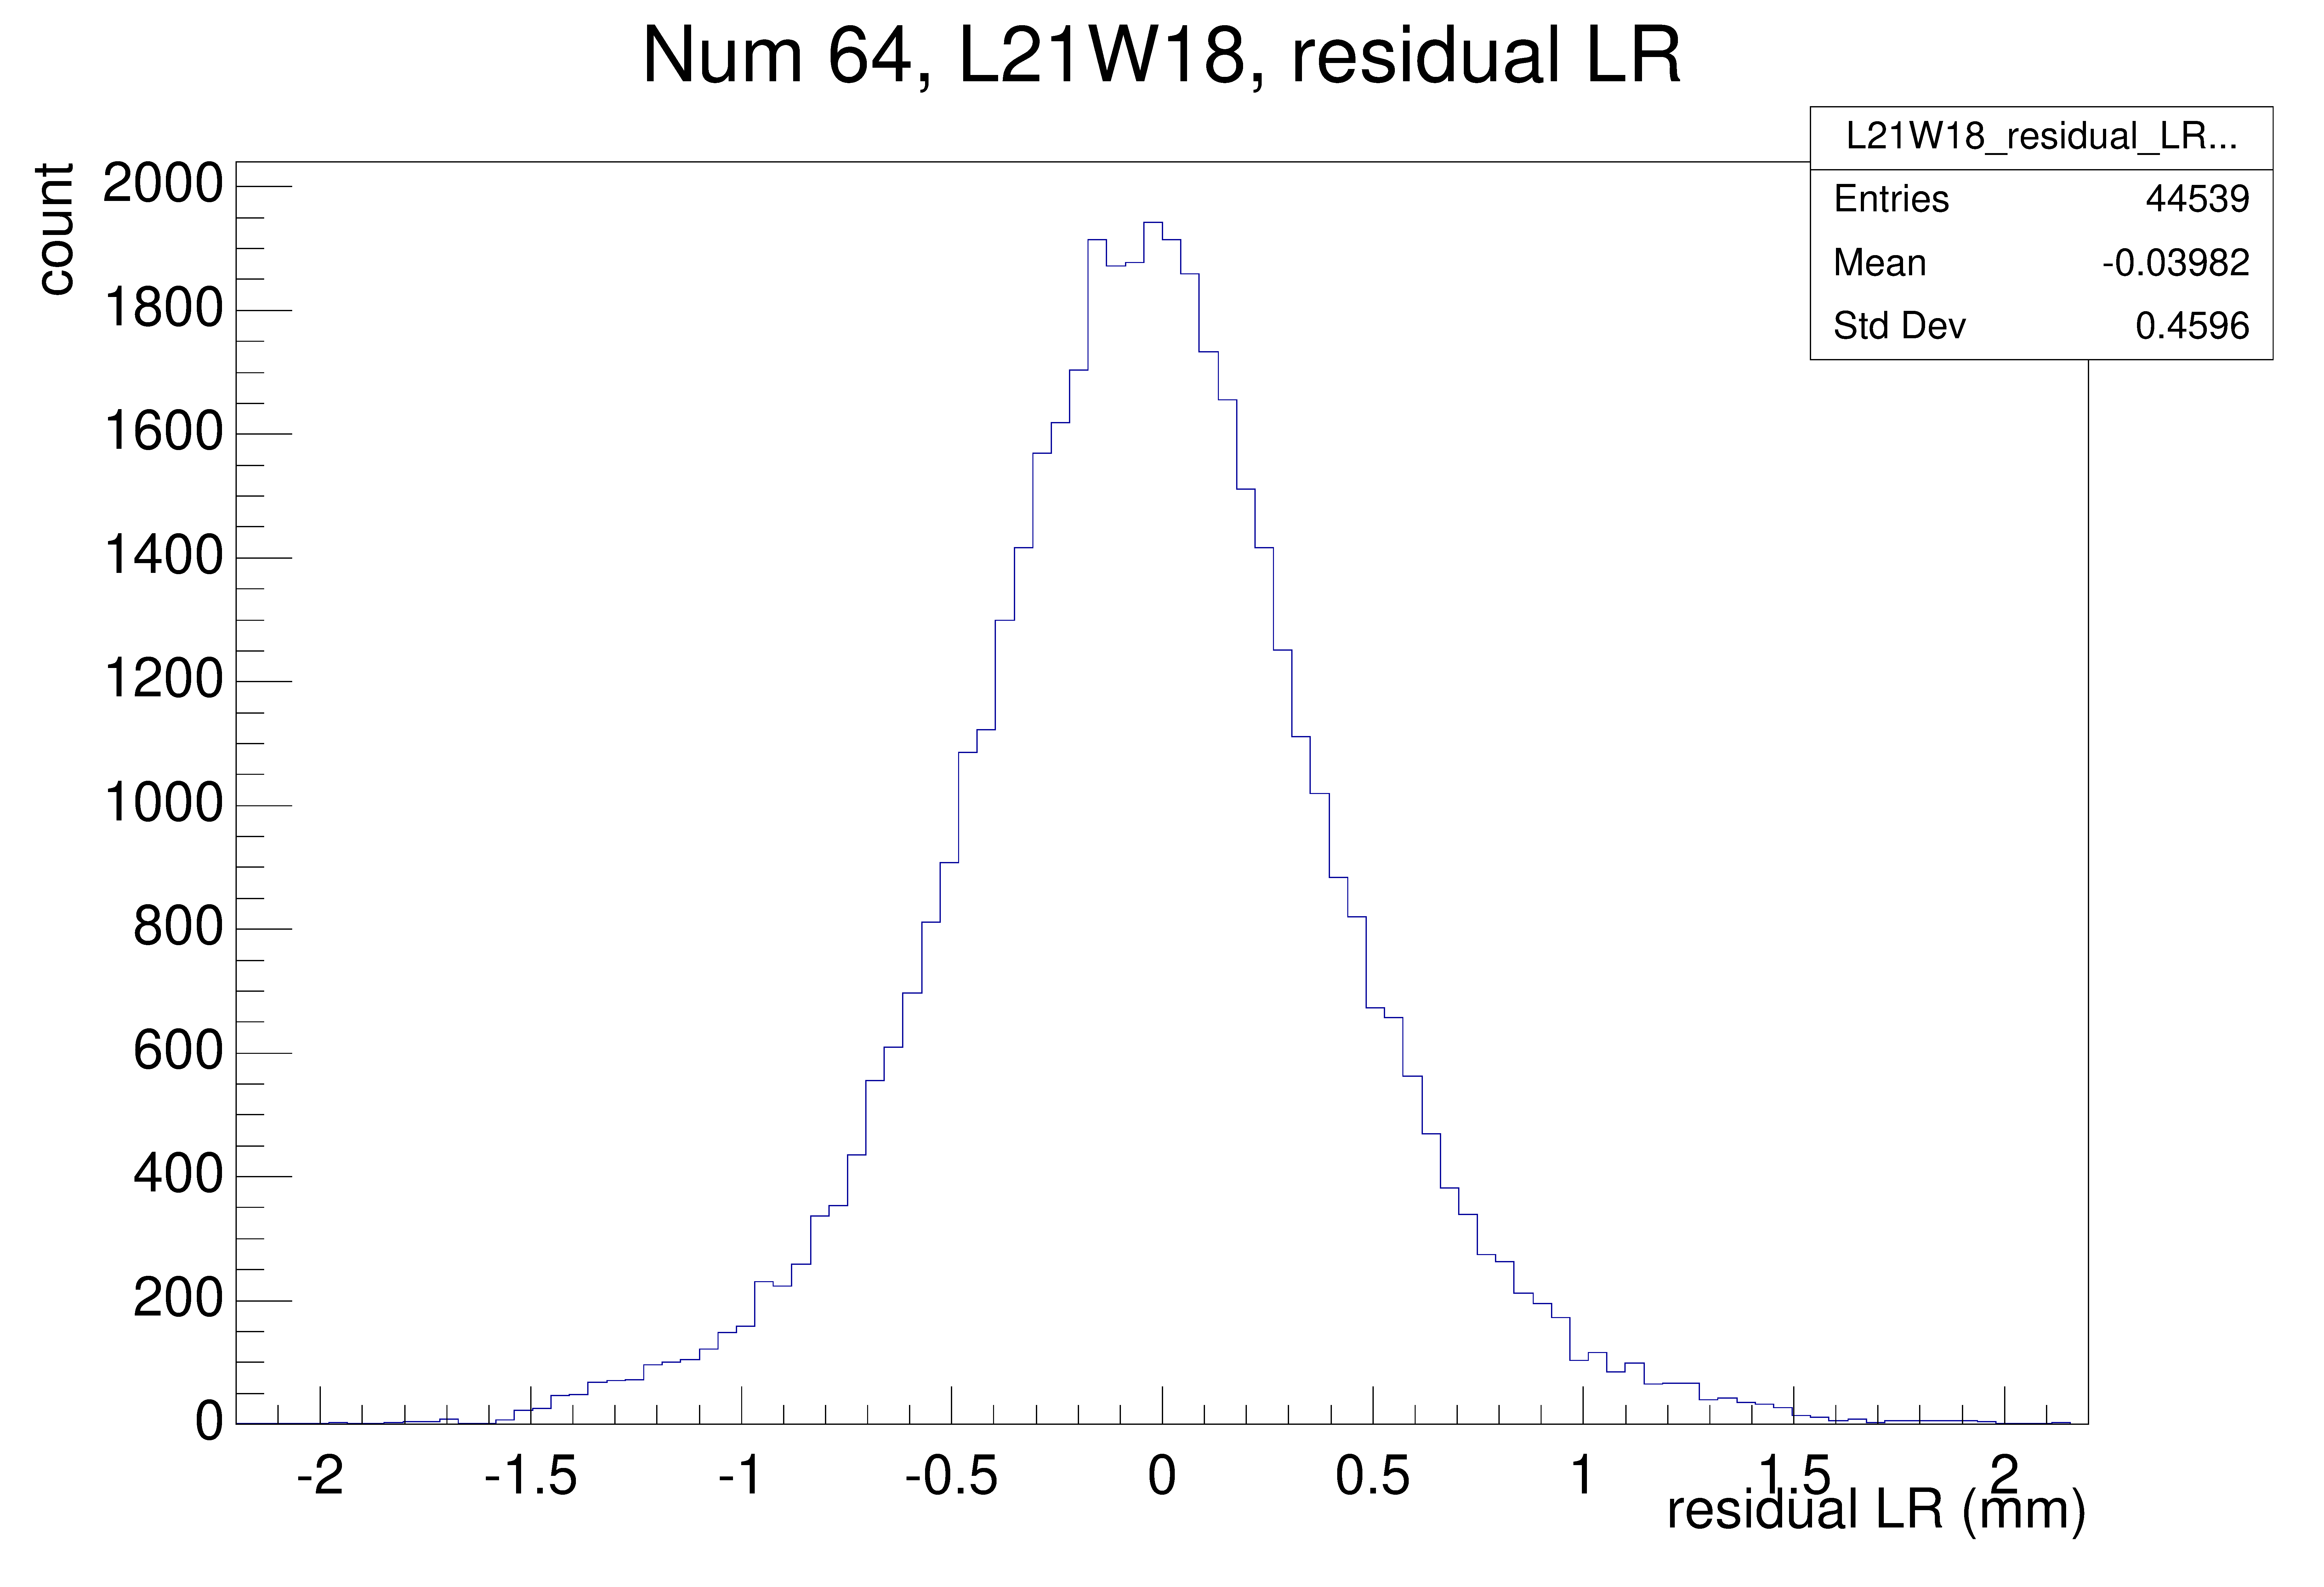
\includegraphics[width=0.20\linewidth]{figures/L21W18_new_tt.pdf} & 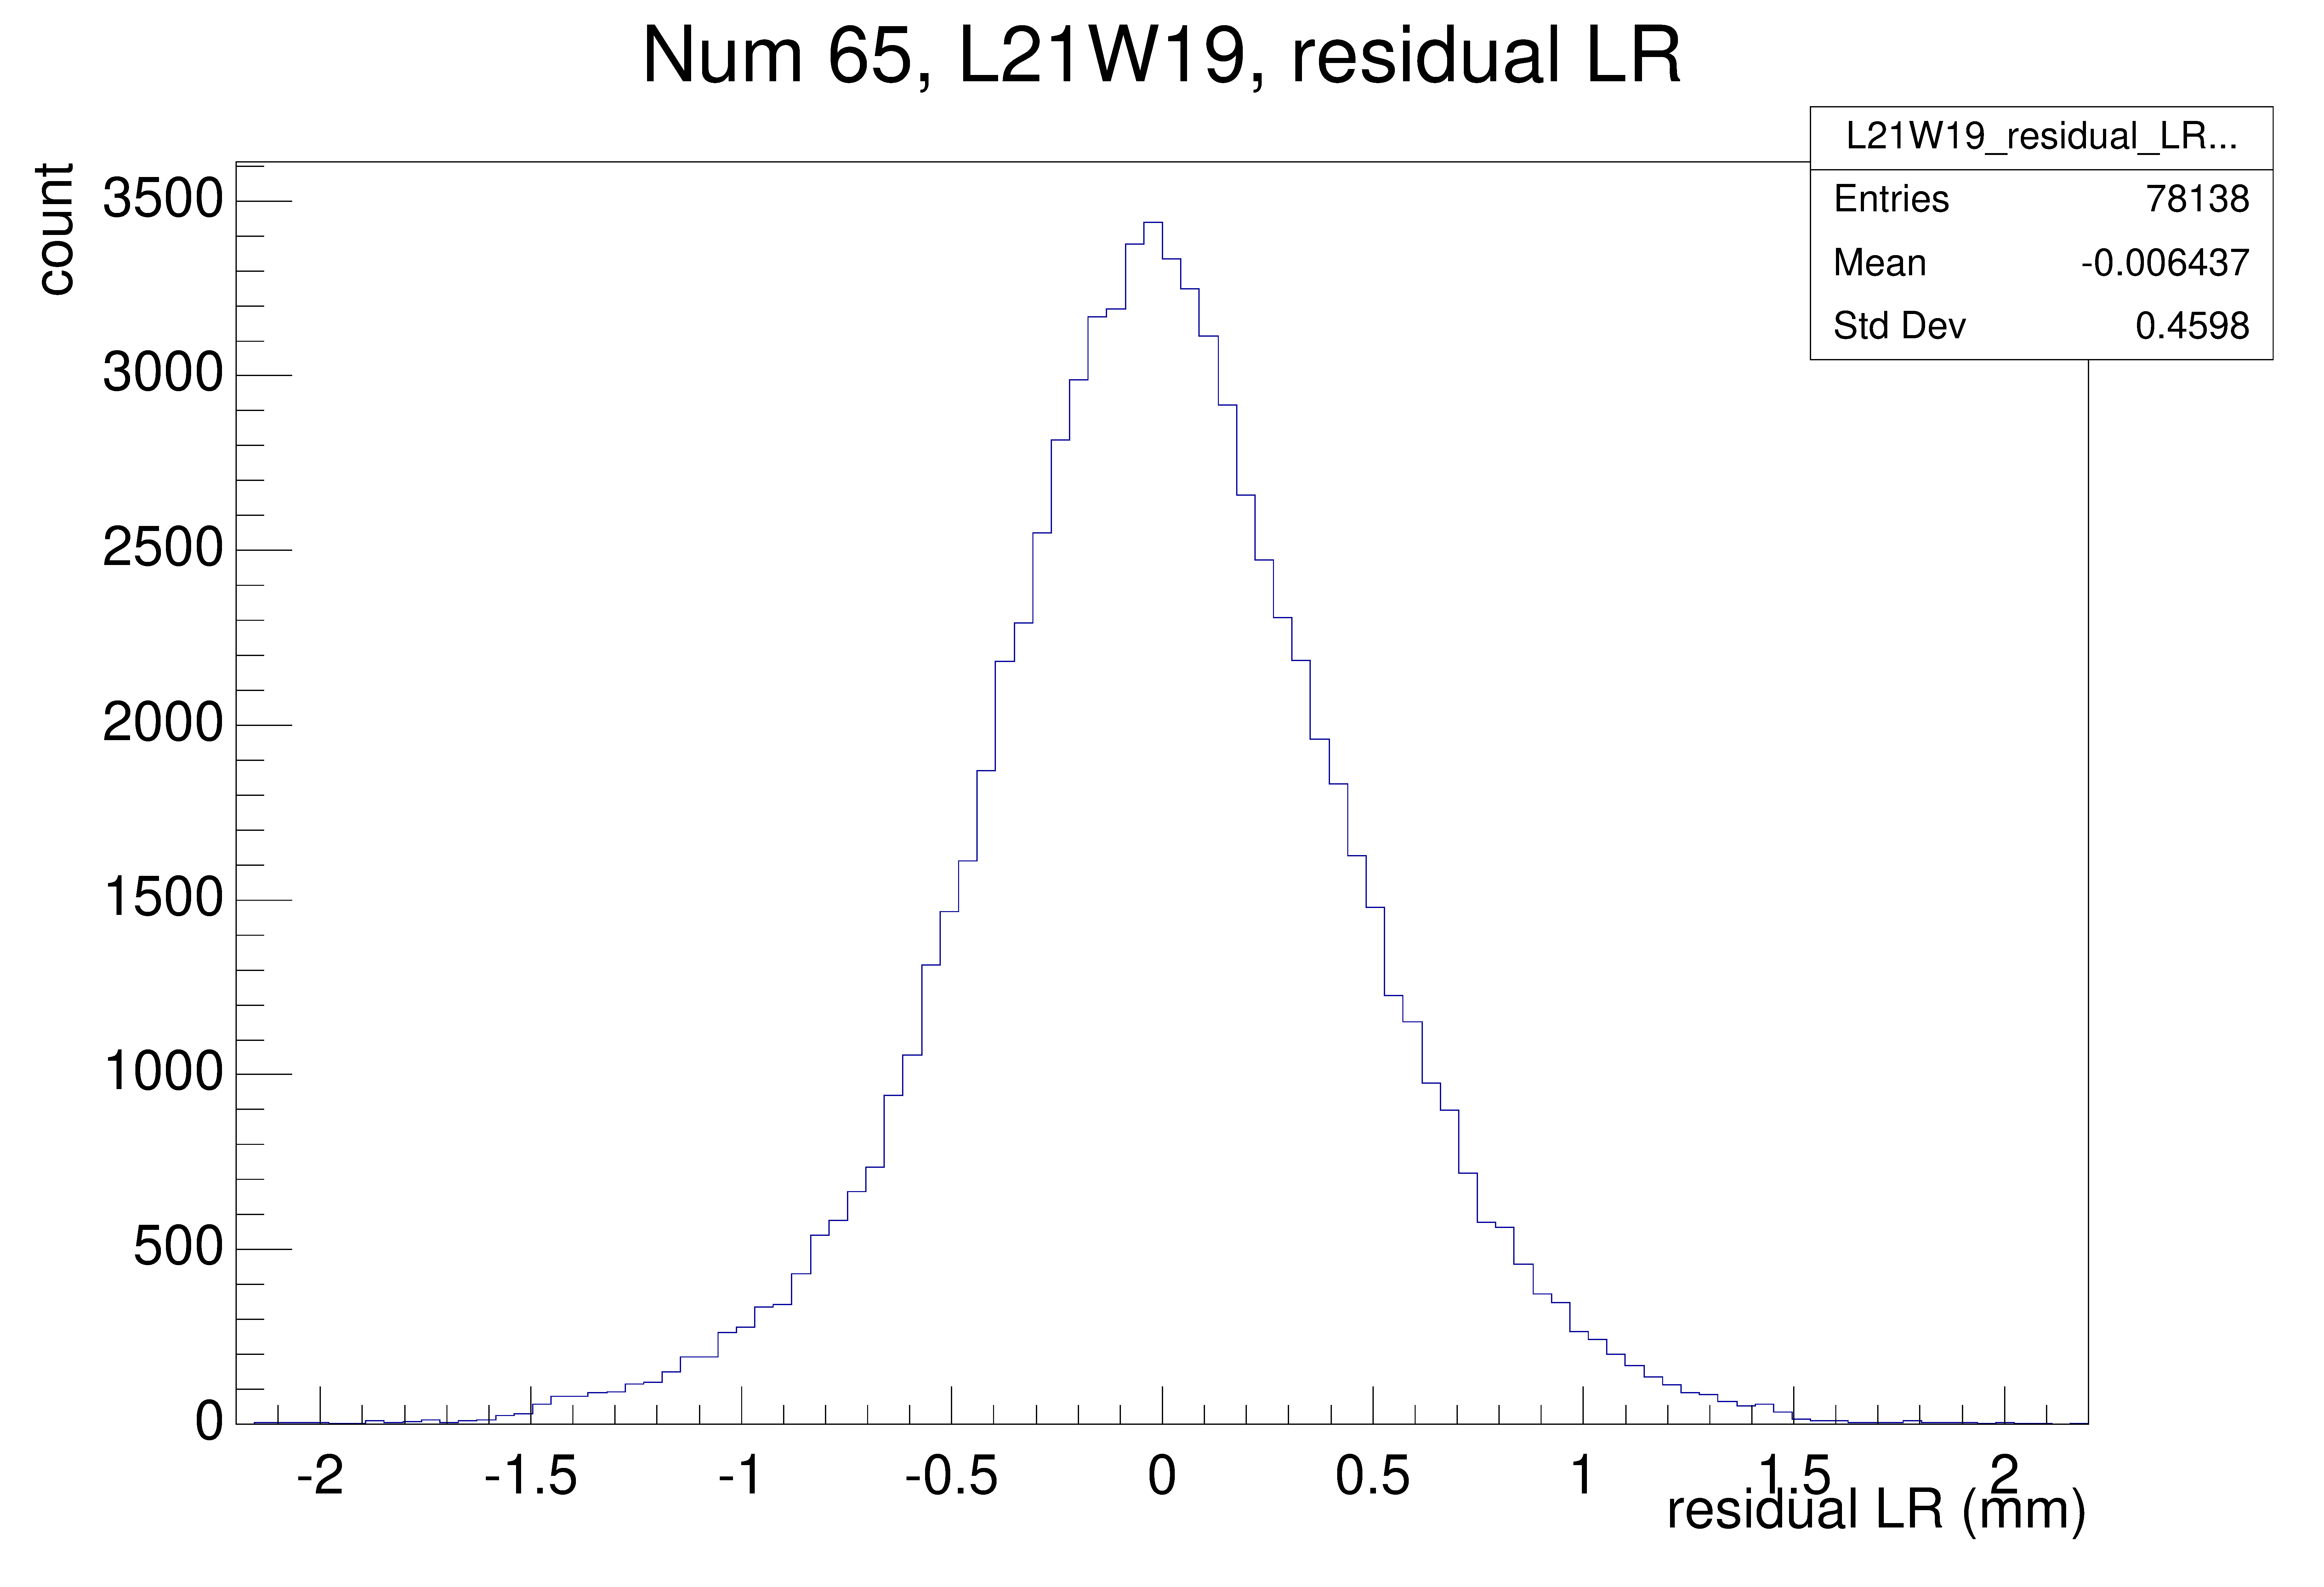
\includegraphics[width=0.20\linewidth]{figures/L21W19_new_tt.pdf} \\

        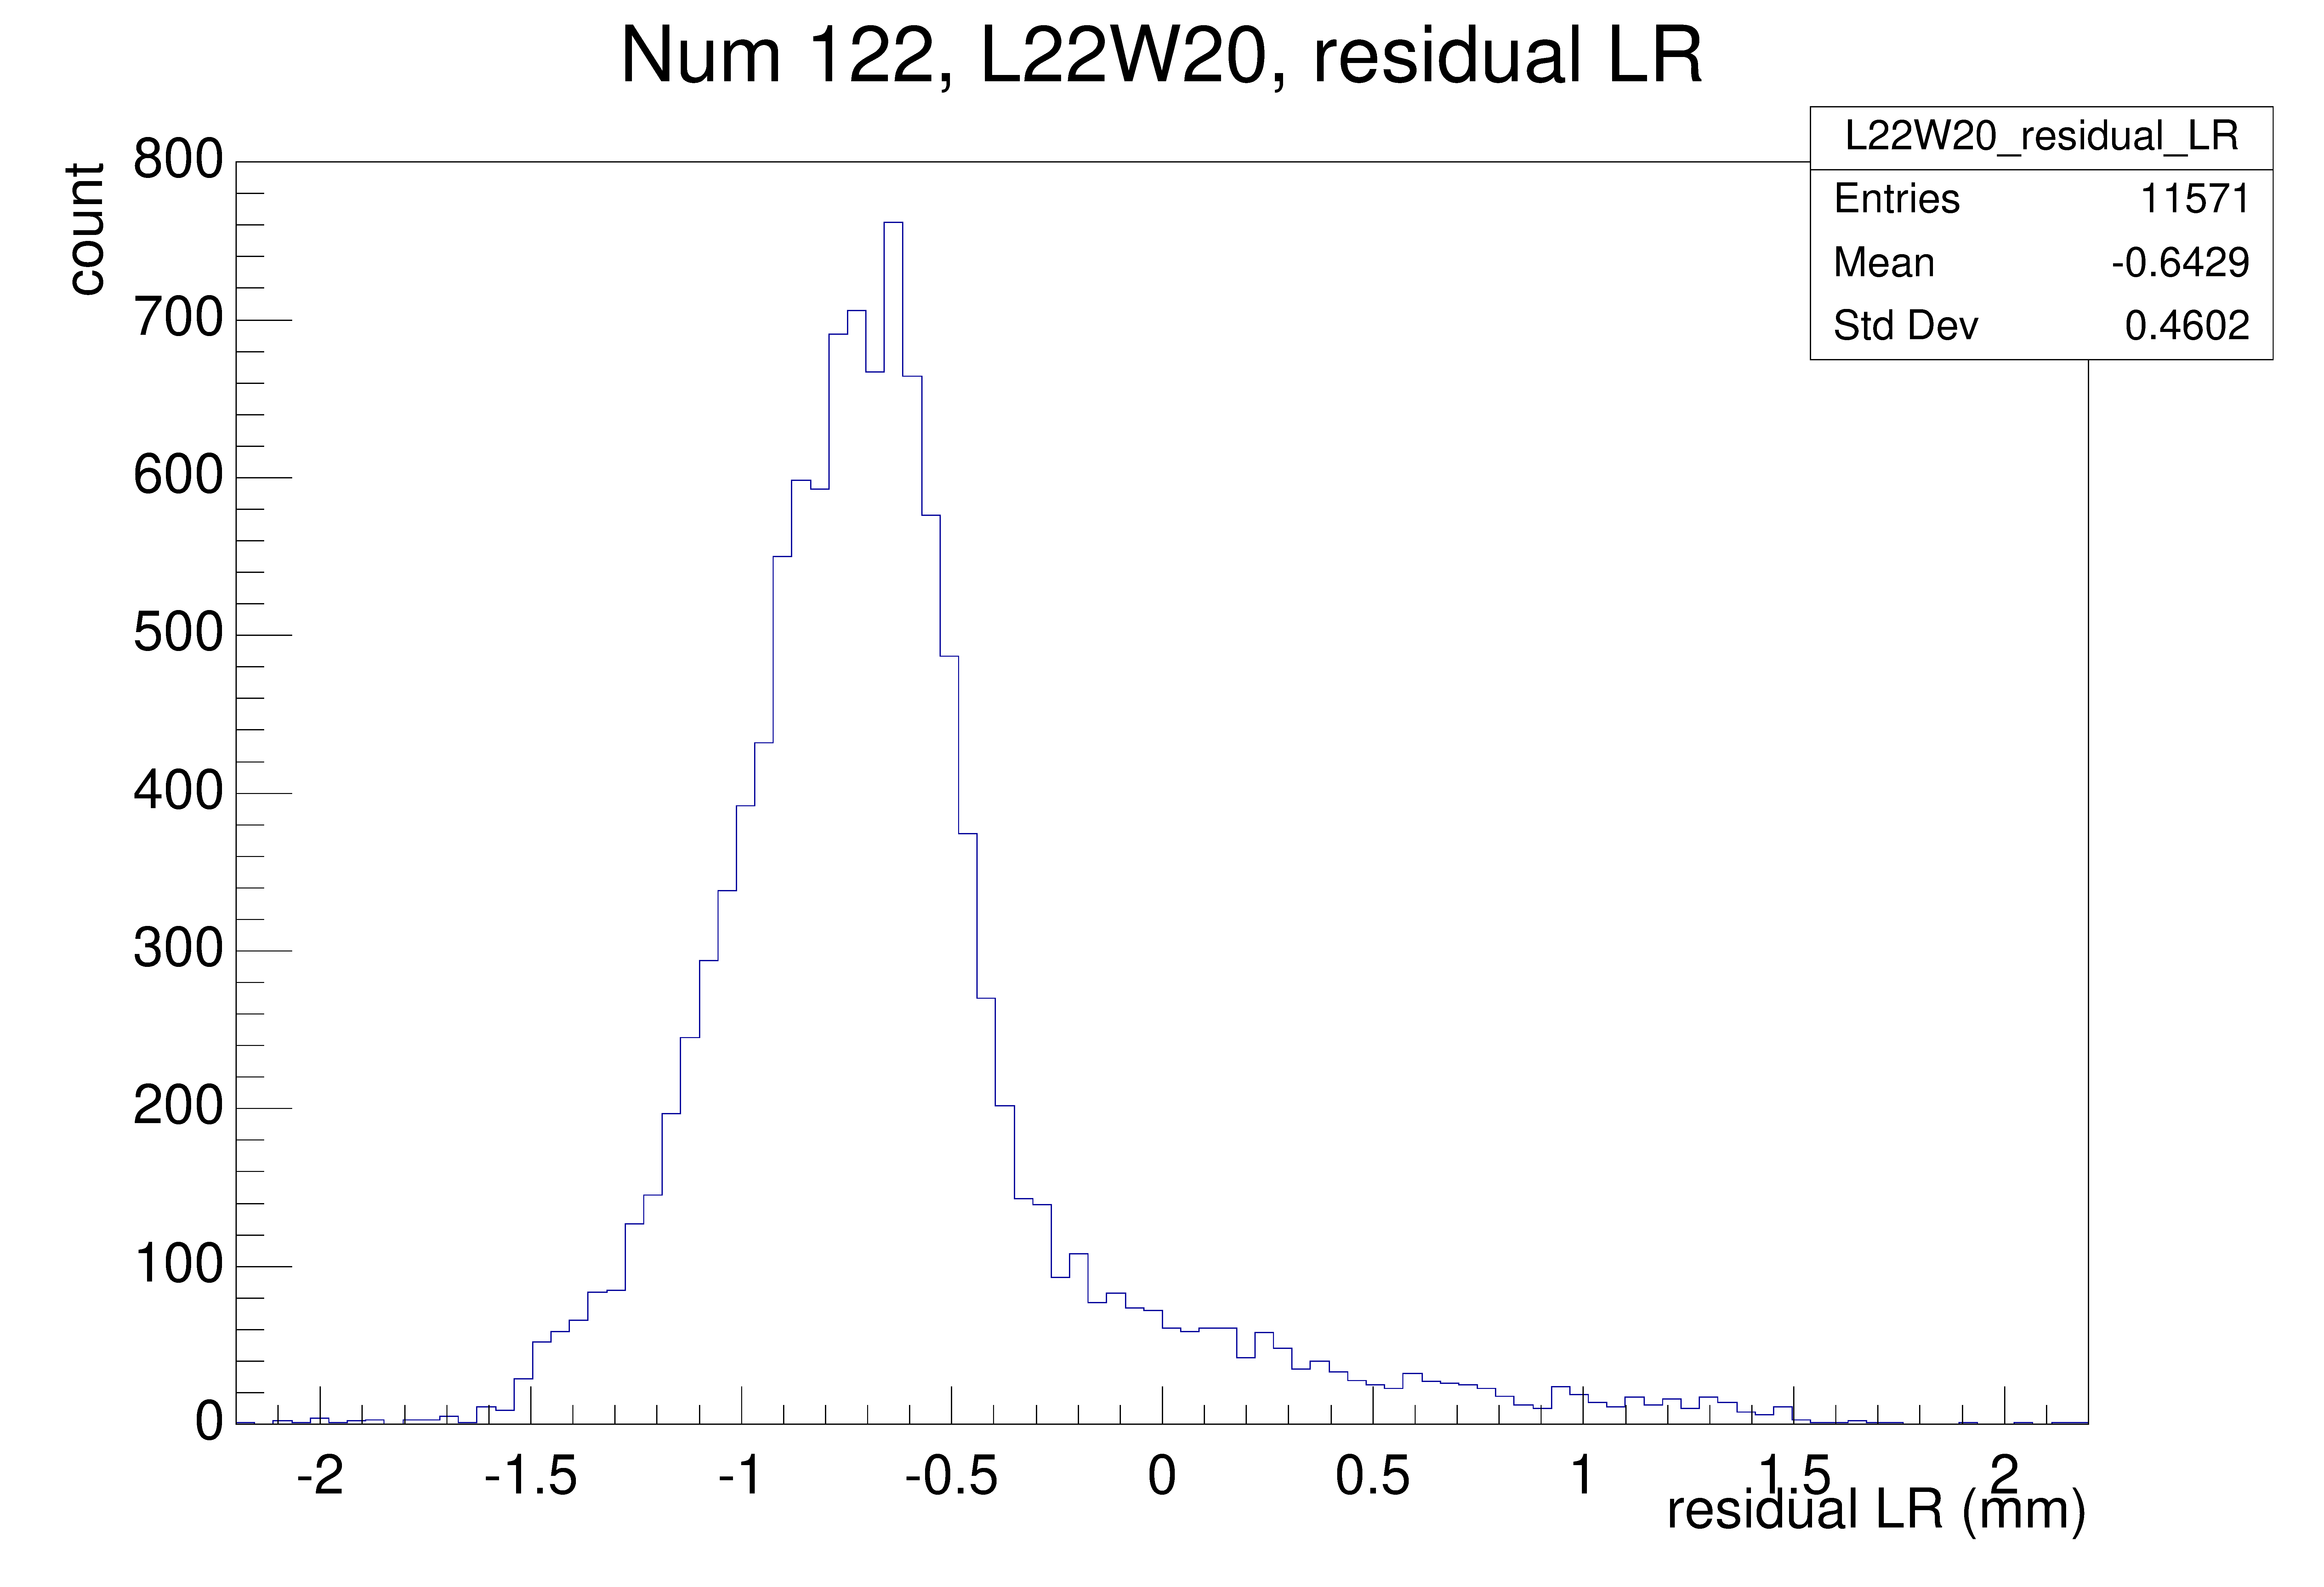
\includegraphics[width=0.20\linewidth]{figures/L22W20_old_tt.pdf} & 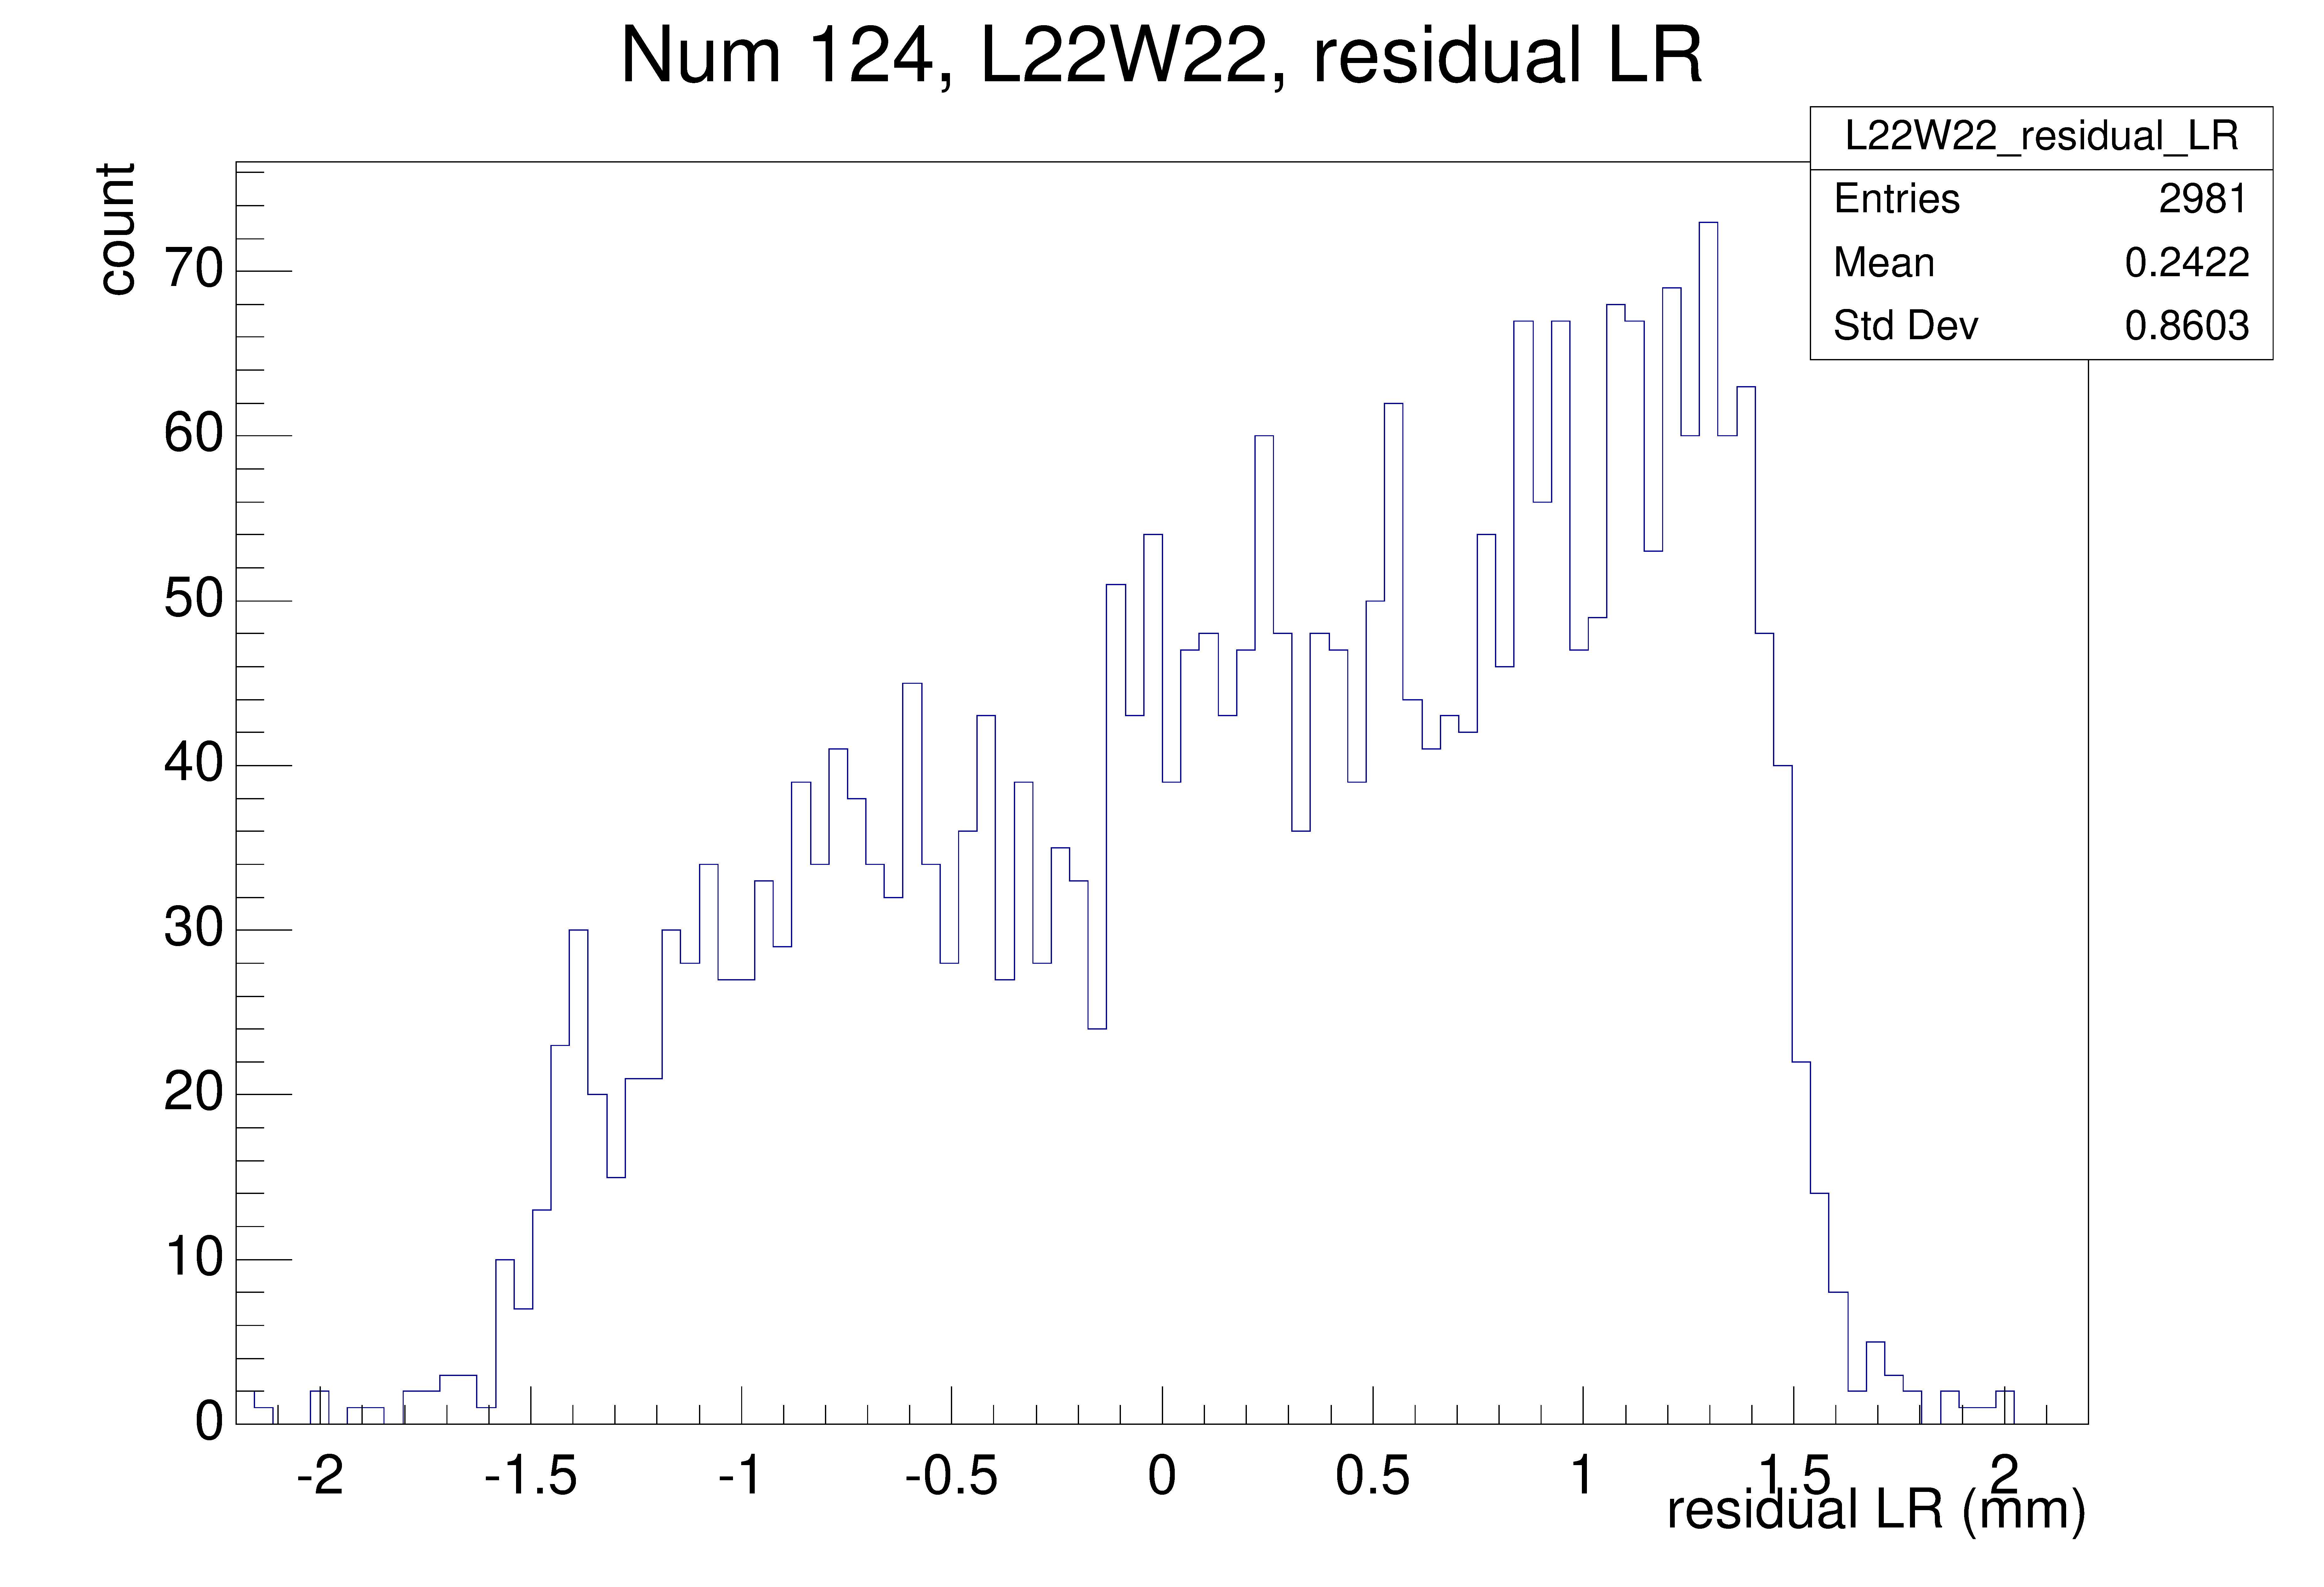
\includegraphics[width=0.20\linewidth]{figures/L22W22_old_tt.pdf} & 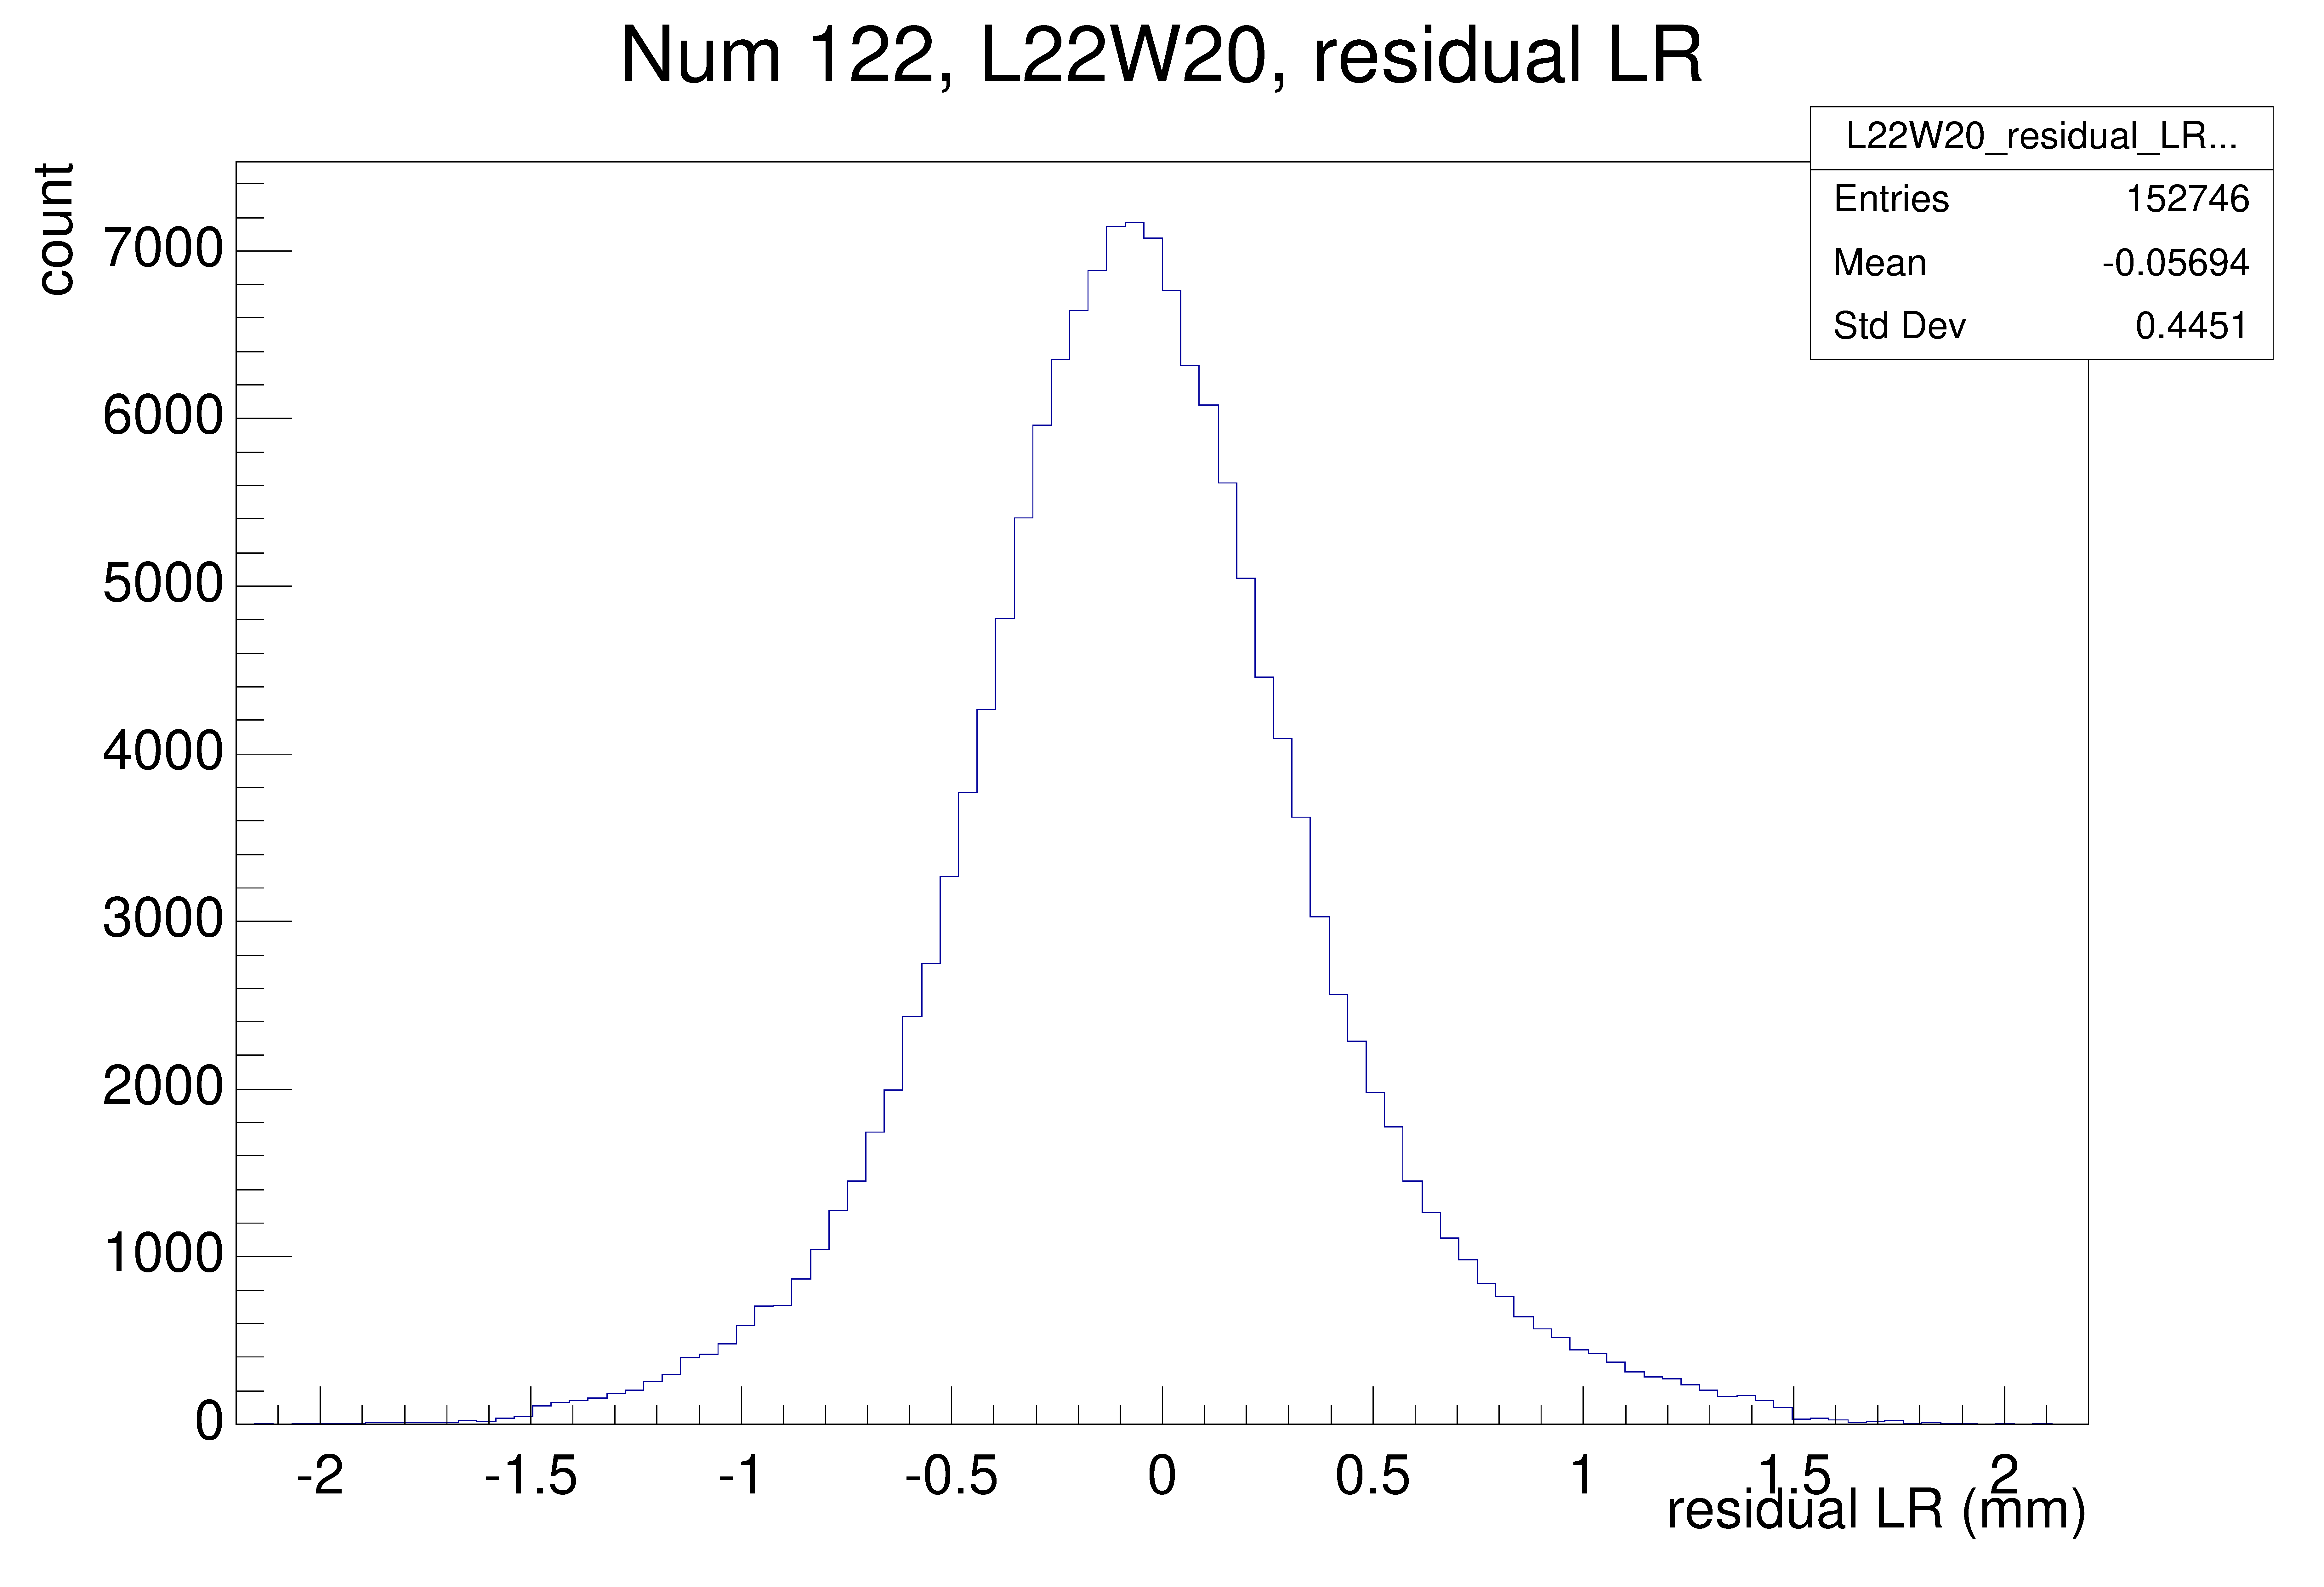
\includegraphics[width=0.20\linewidth]{figures/L22W20_new_tt.pdf} & 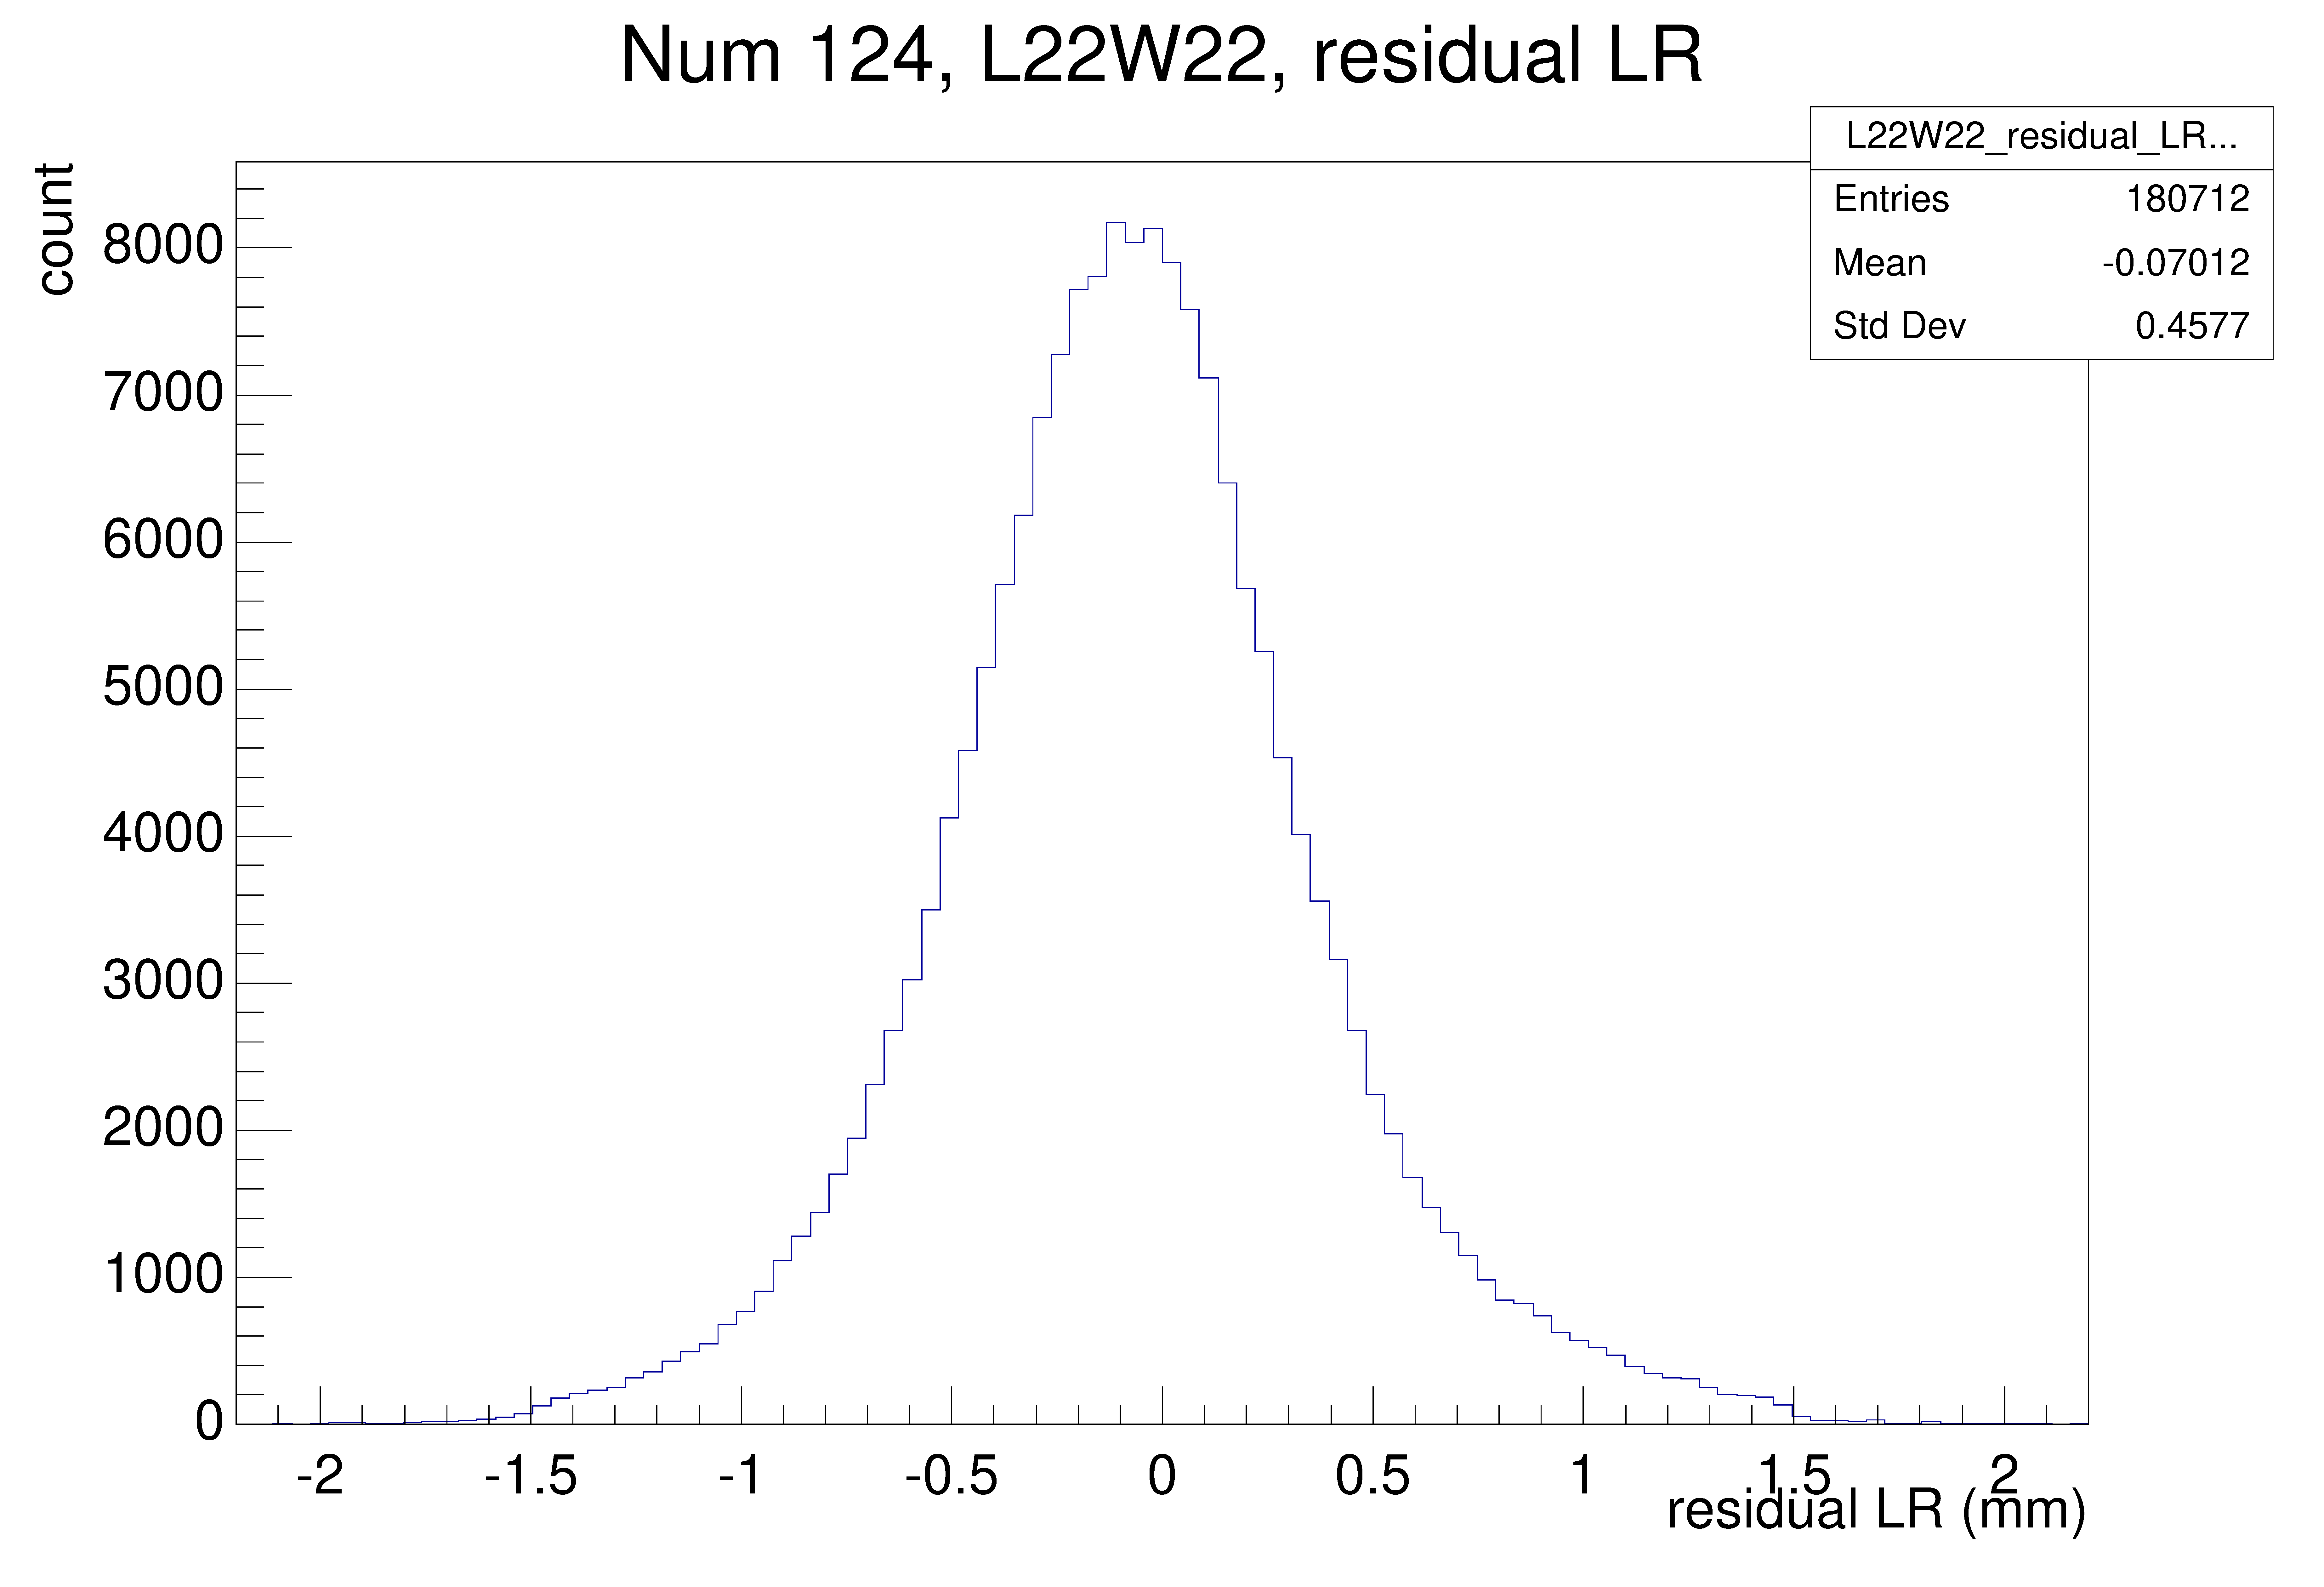
\includegraphics[width=0.20\linewidth]{figures/L22W22_new_tt.pdf} \\

        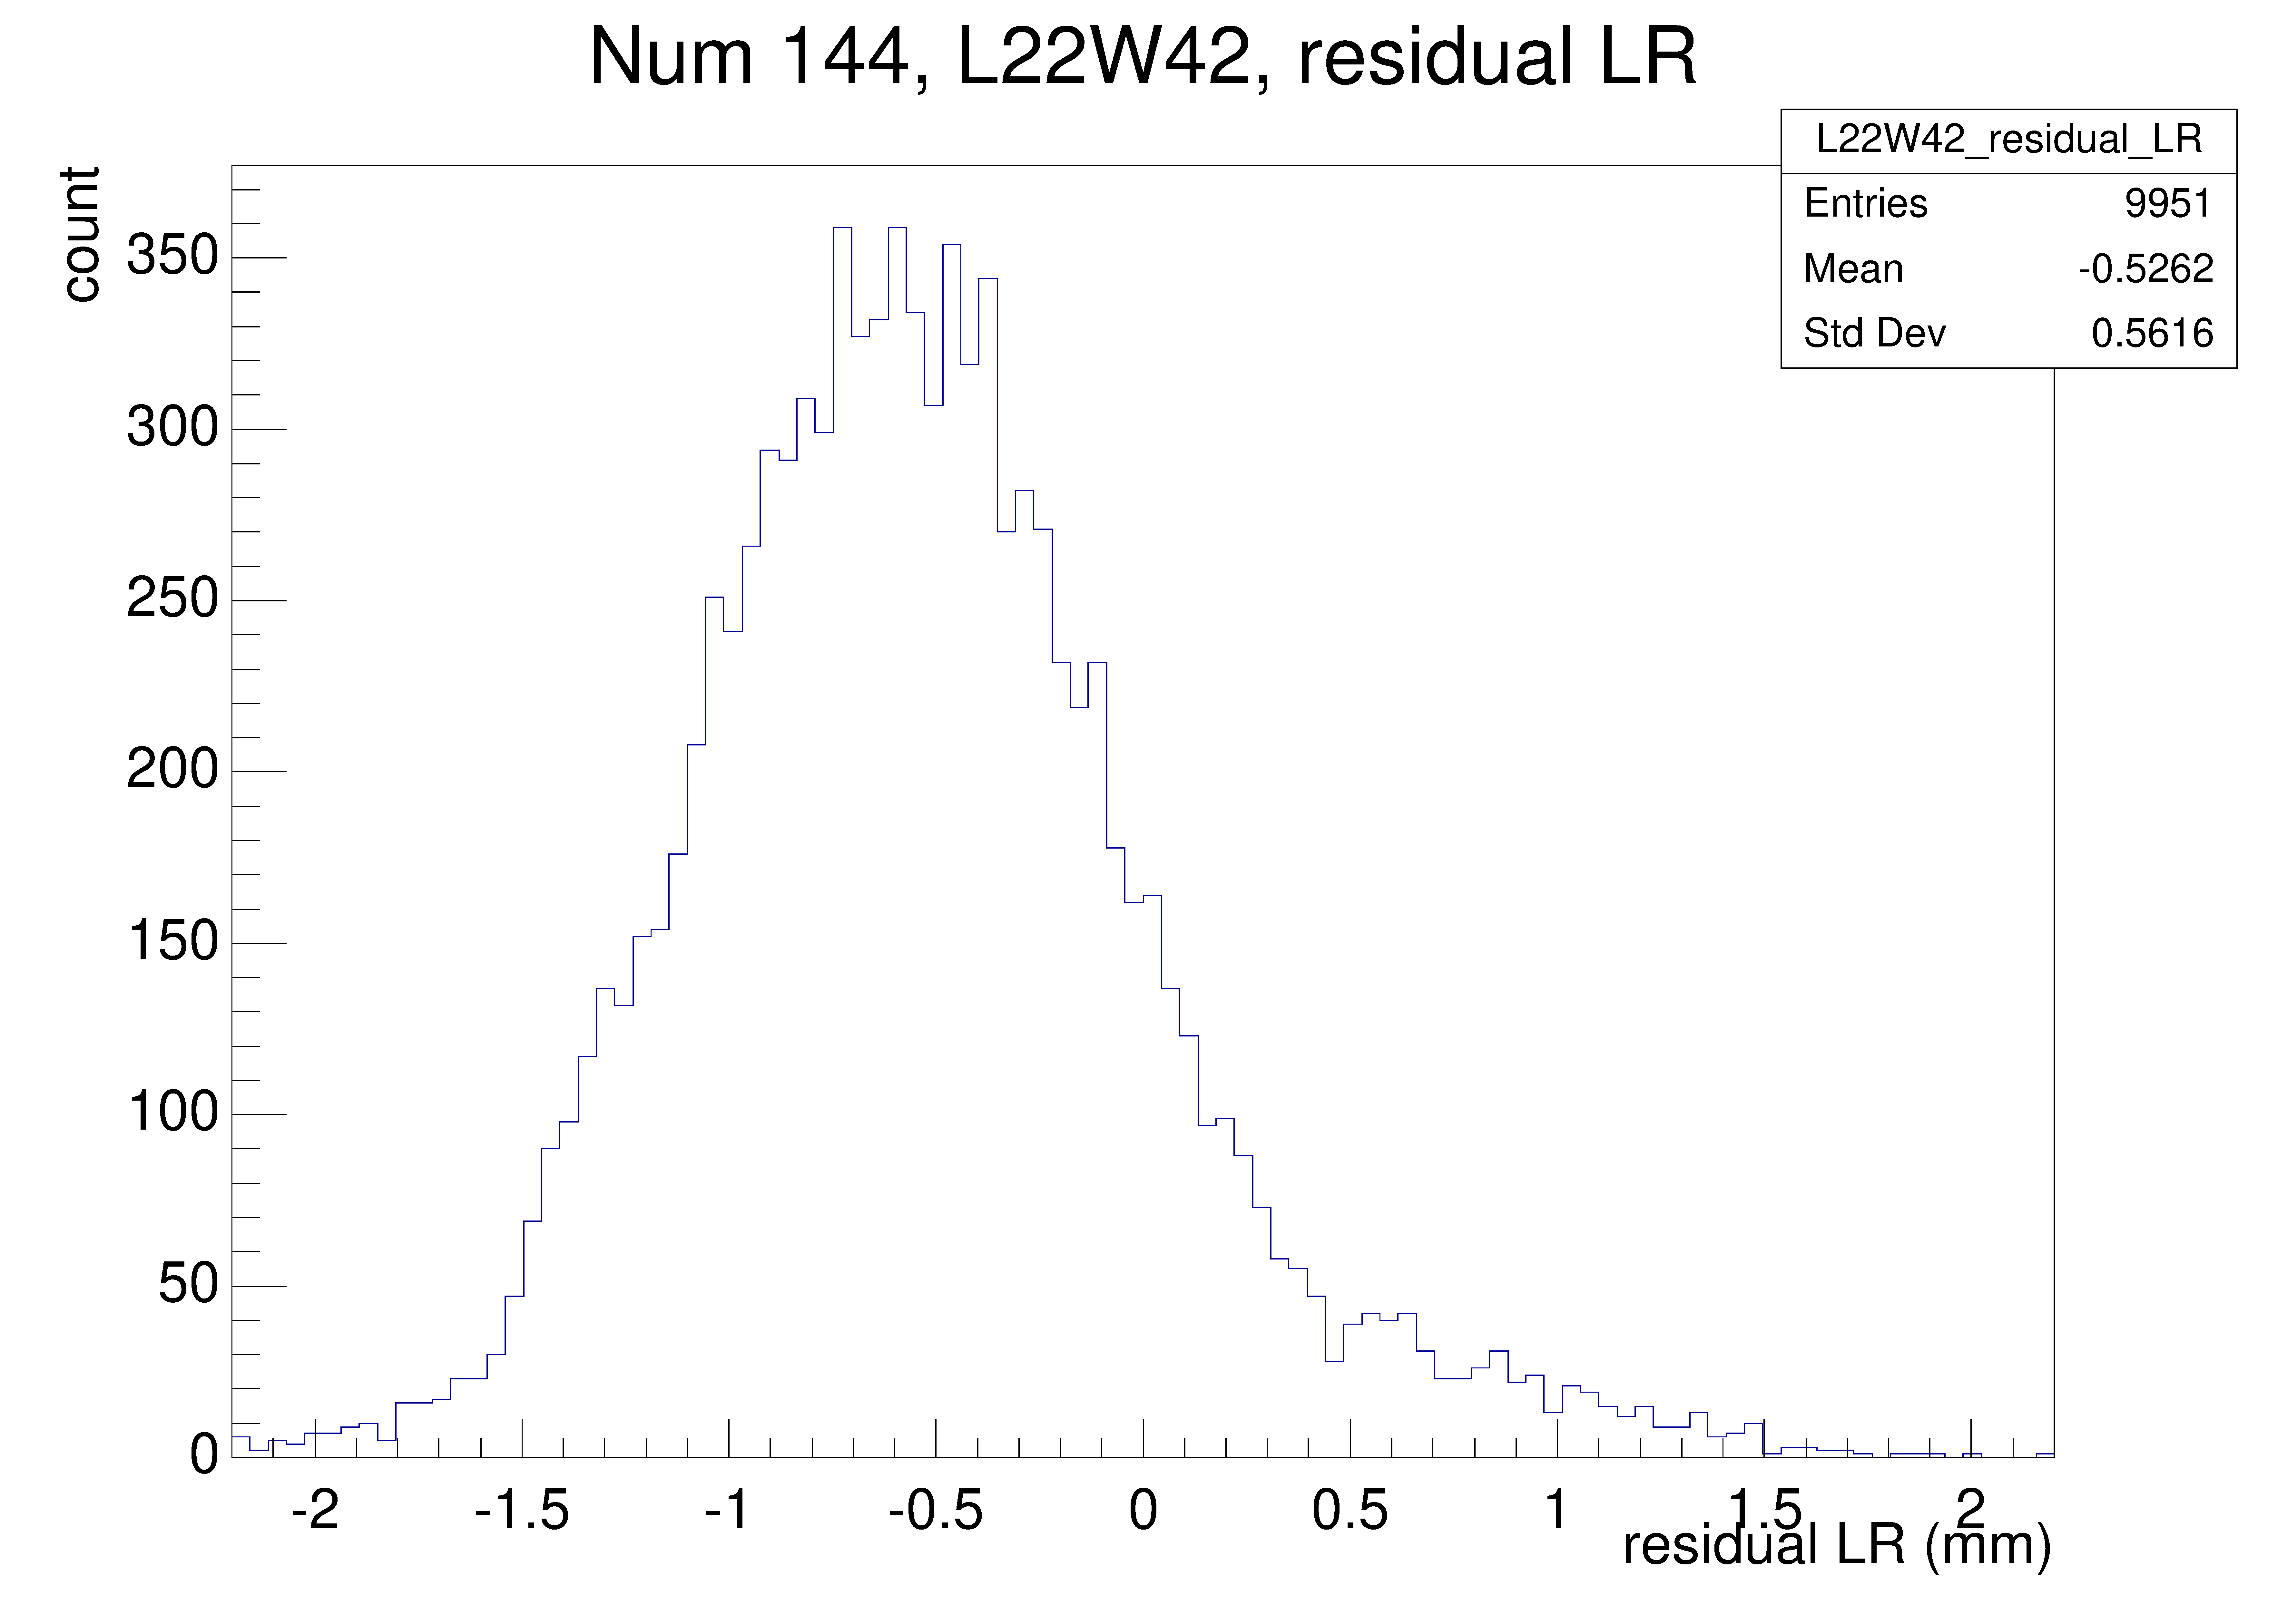
\includegraphics[width=0.20\linewidth]{figures/L22W42_old_tt.pdf} & 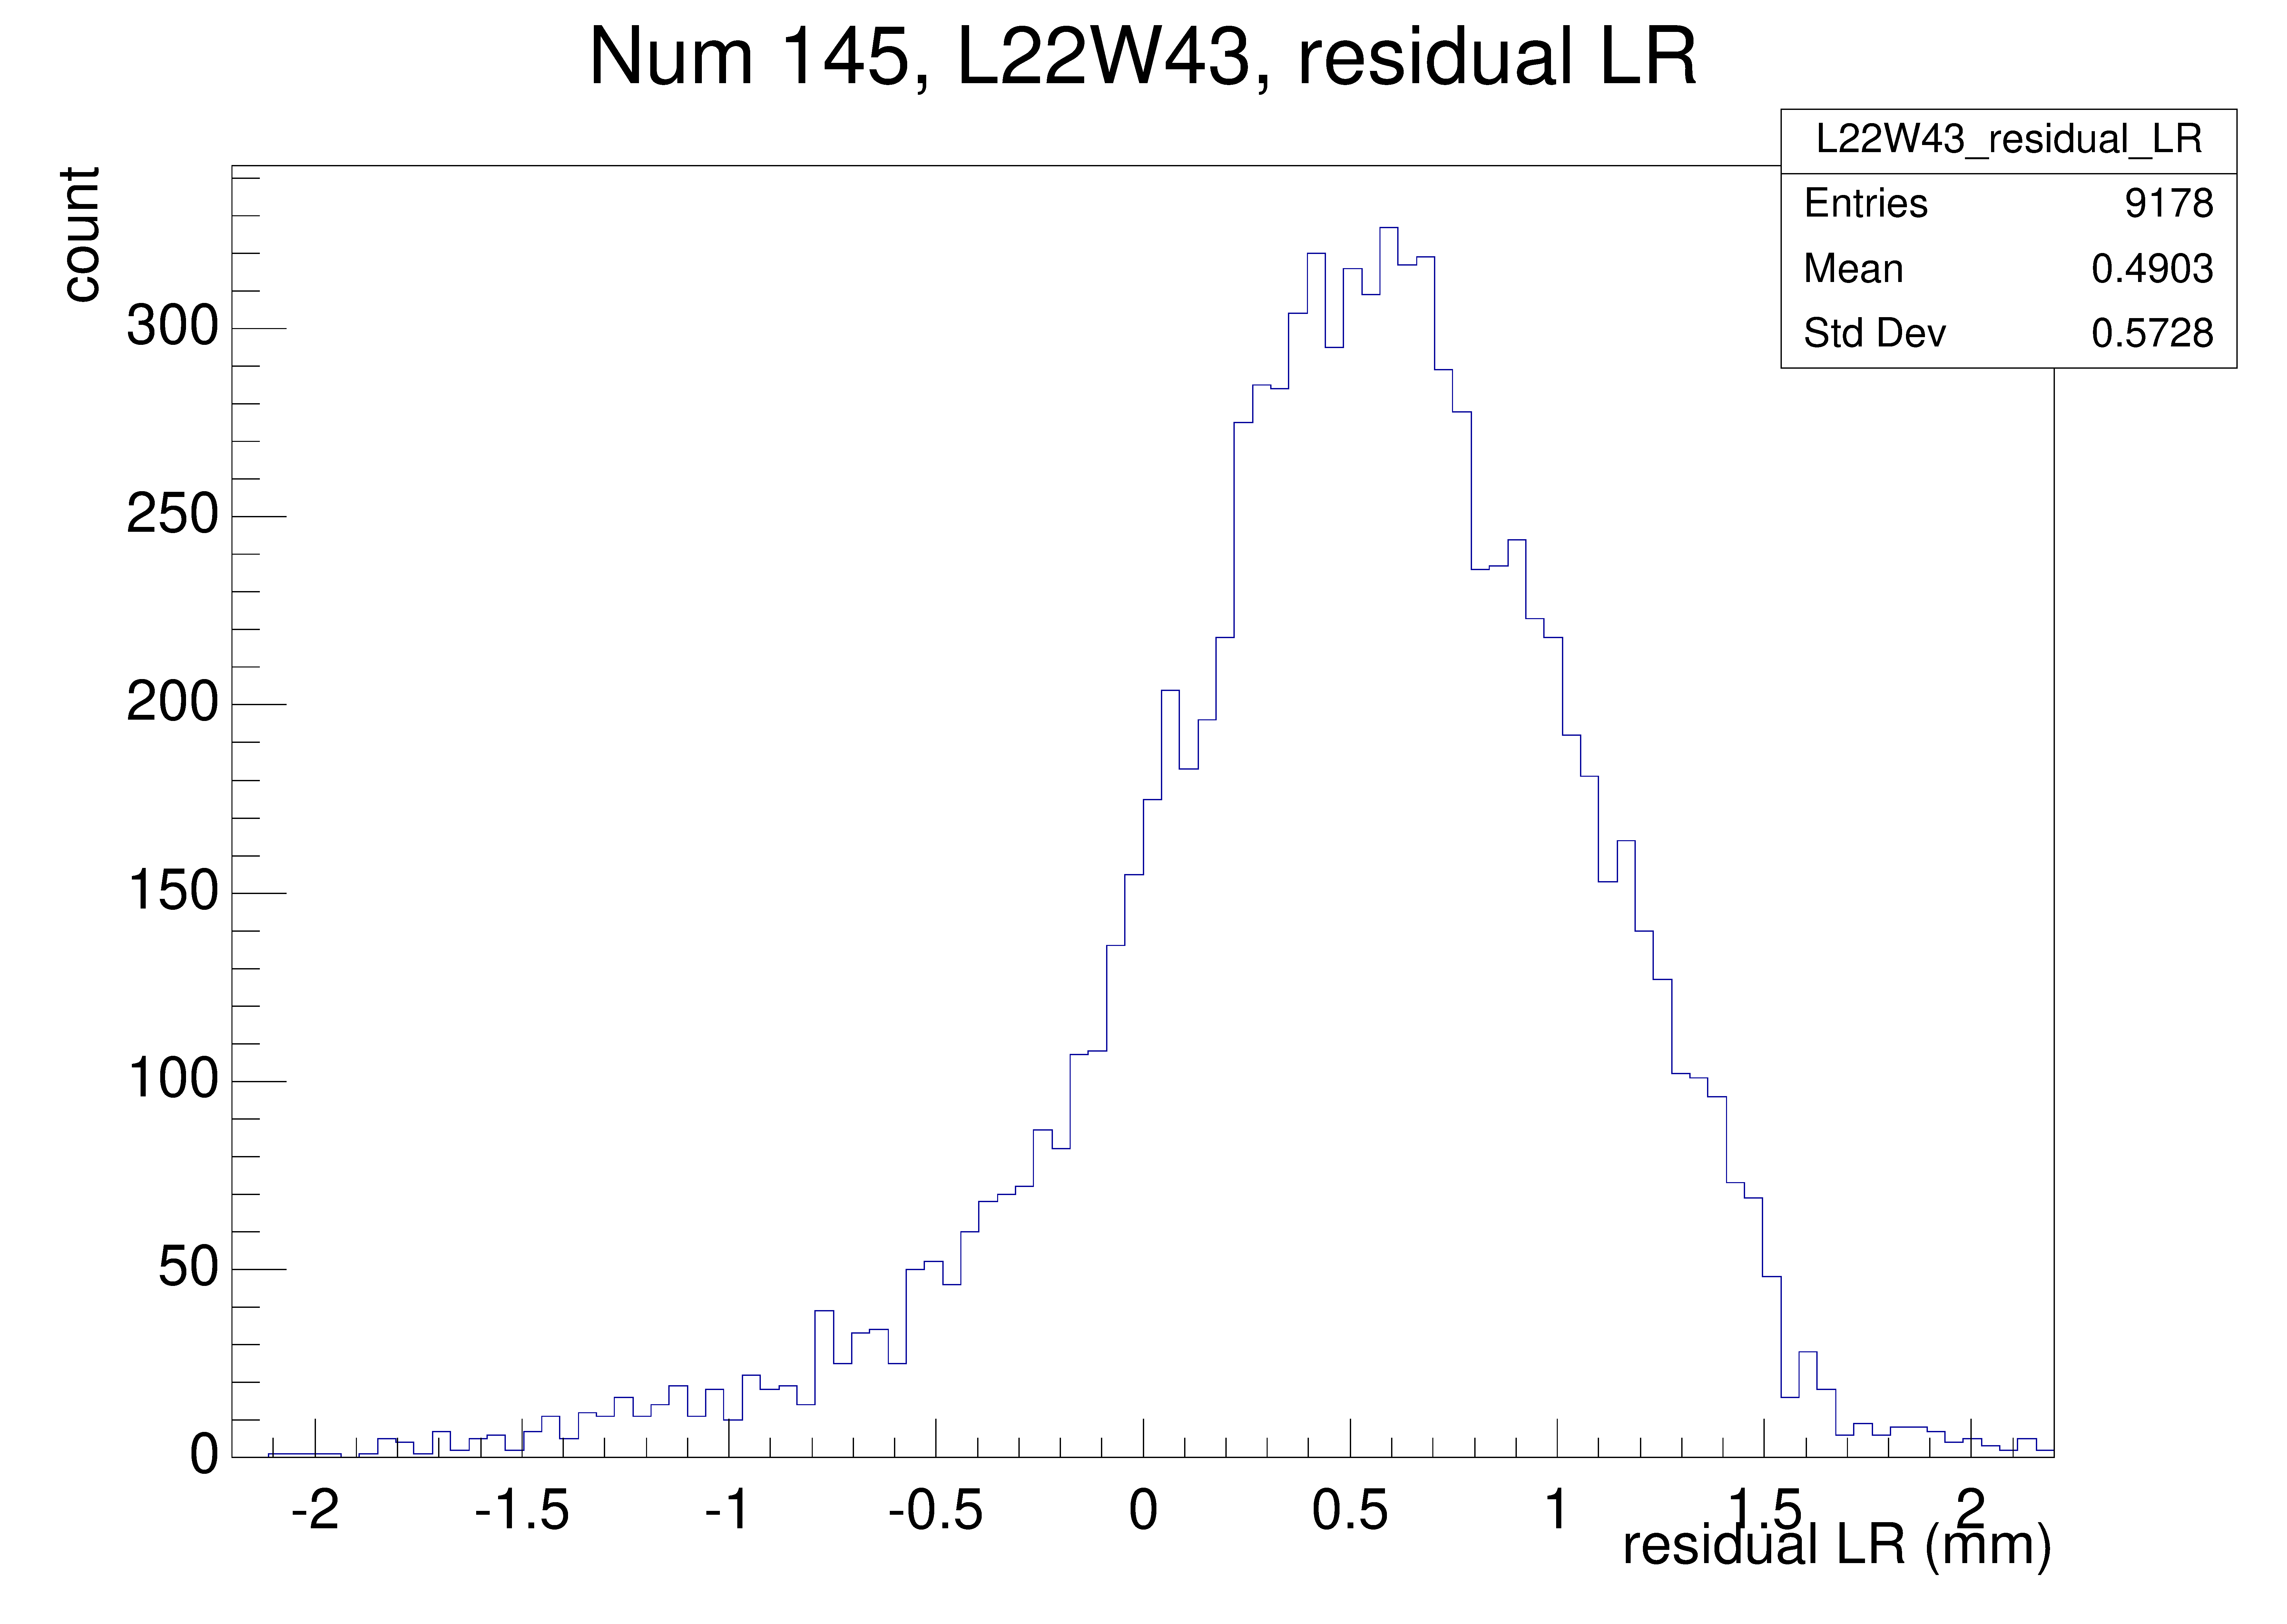
\includegraphics[width=0.20\linewidth]{figures/L22W43_old_tt.pdf} & 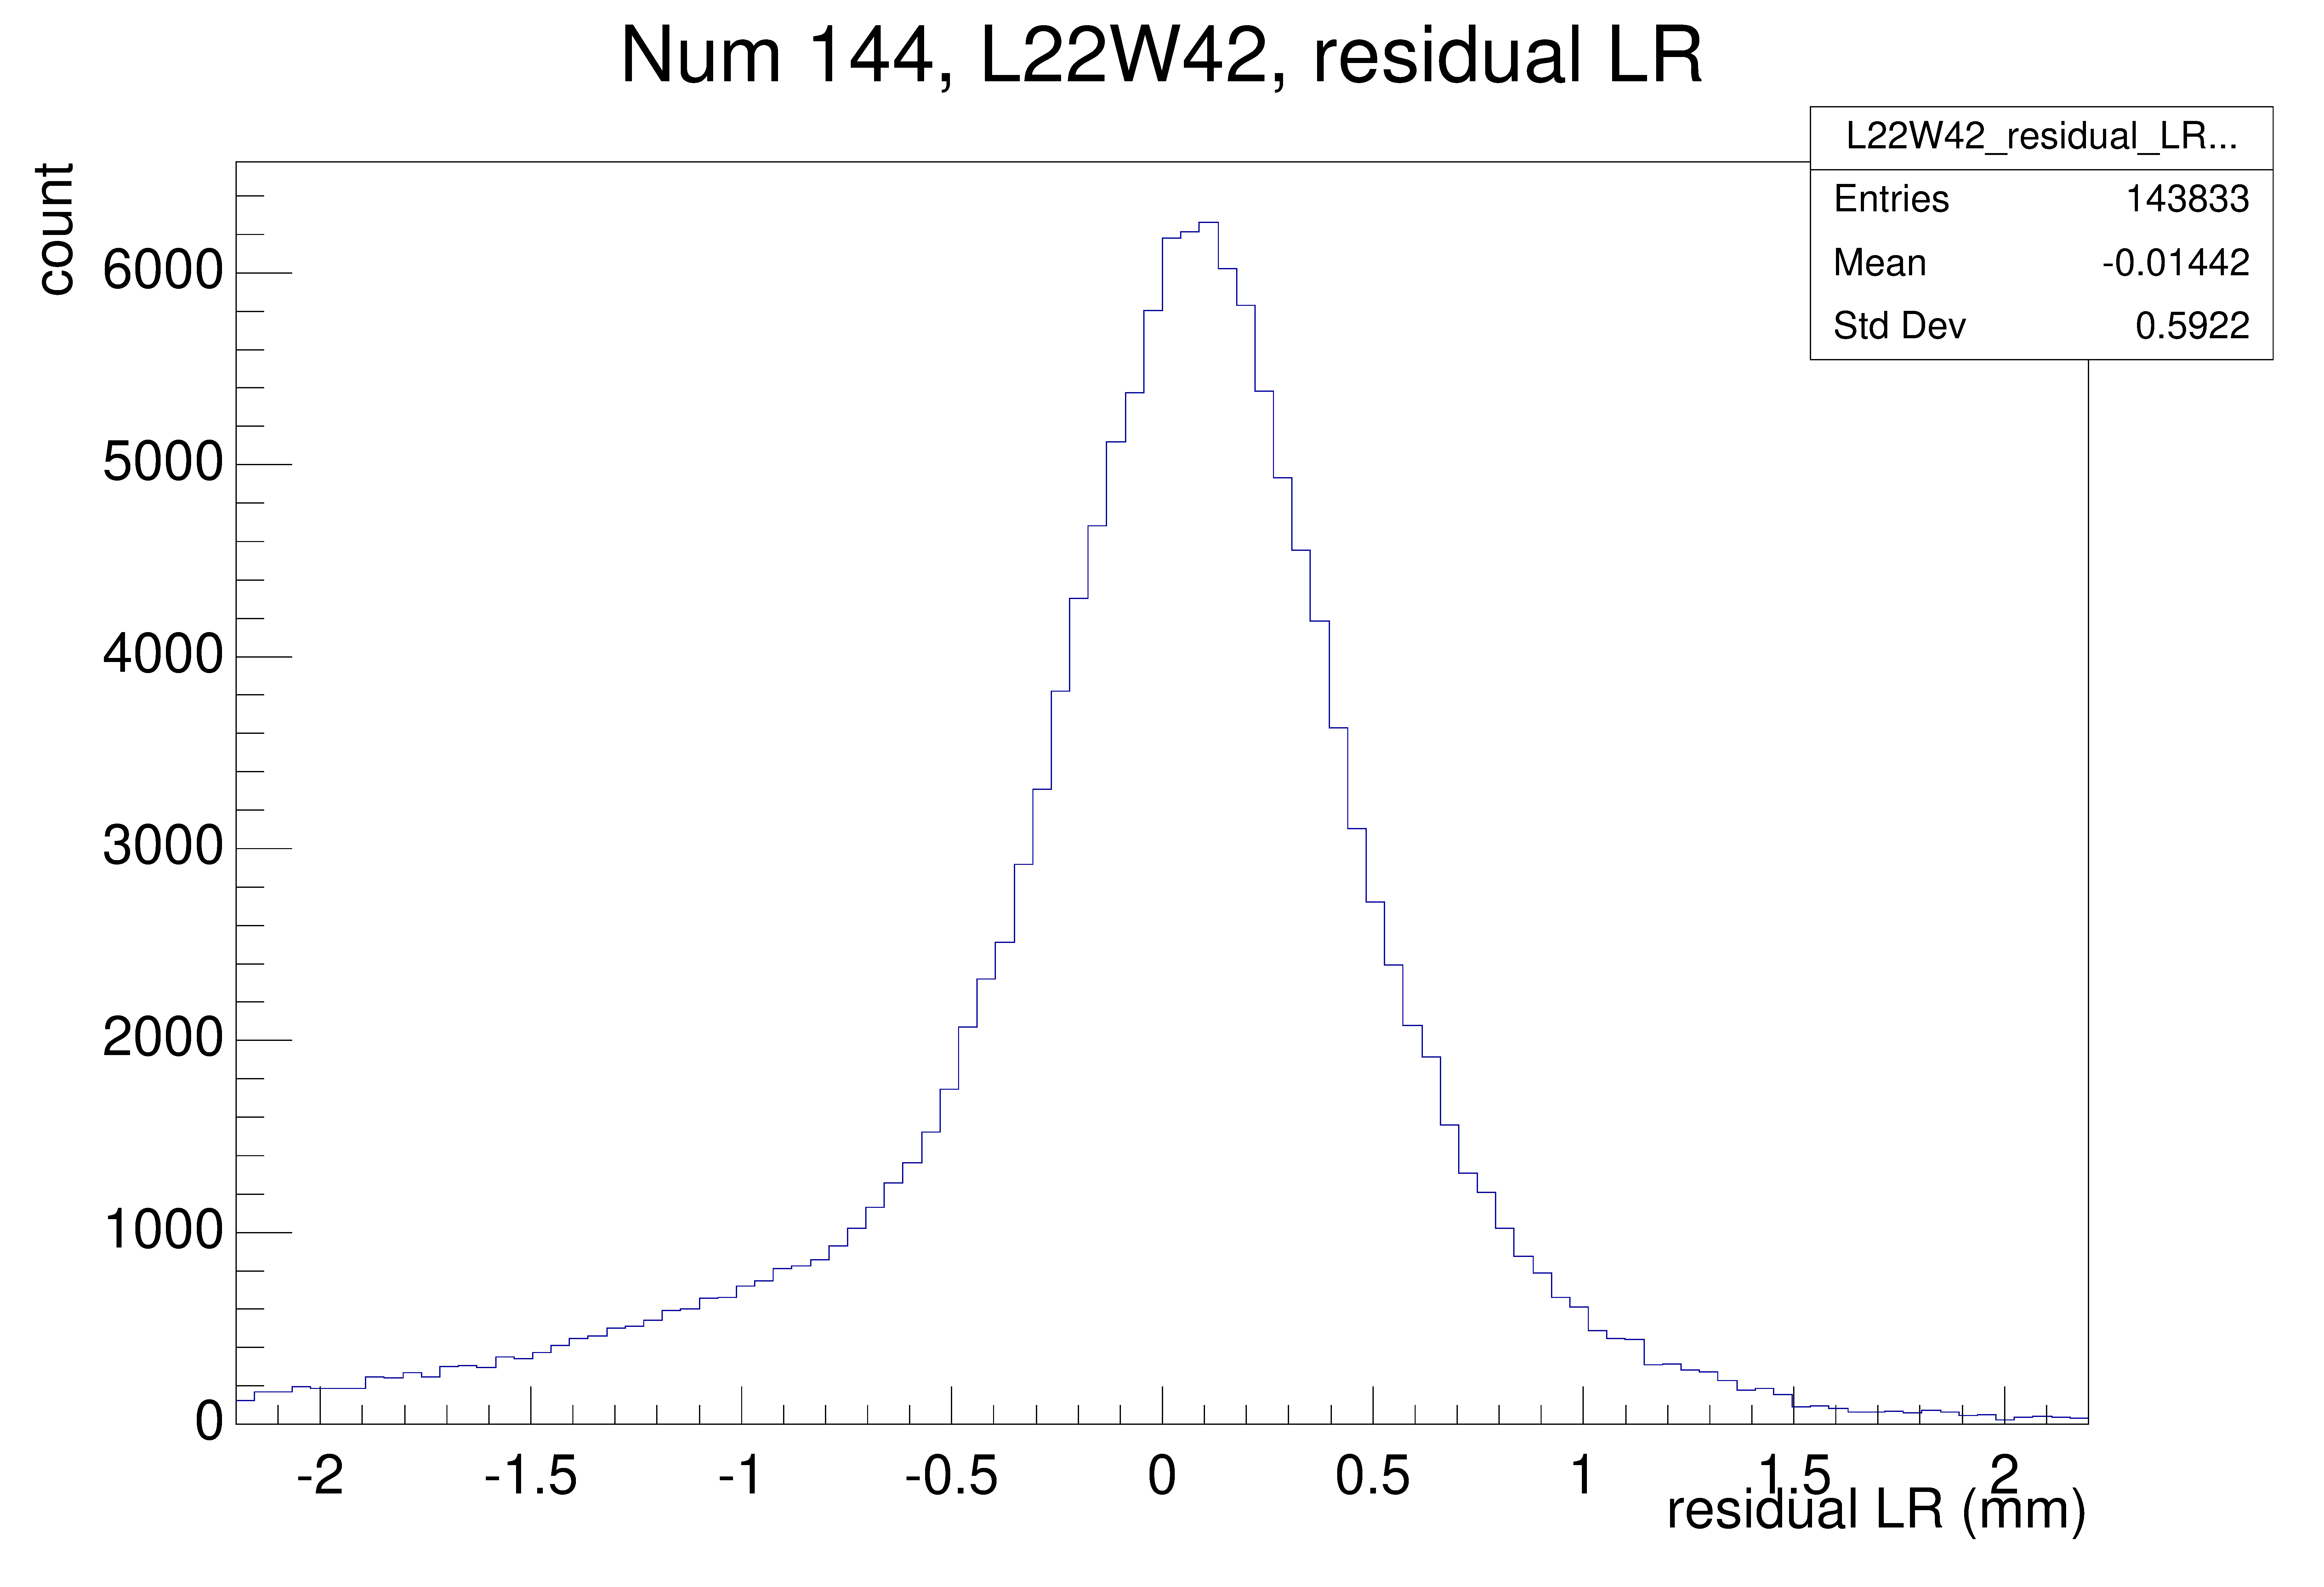
\includegraphics[width=0.20\linewidth]{figures/L22W42_new_tt.pdf} & 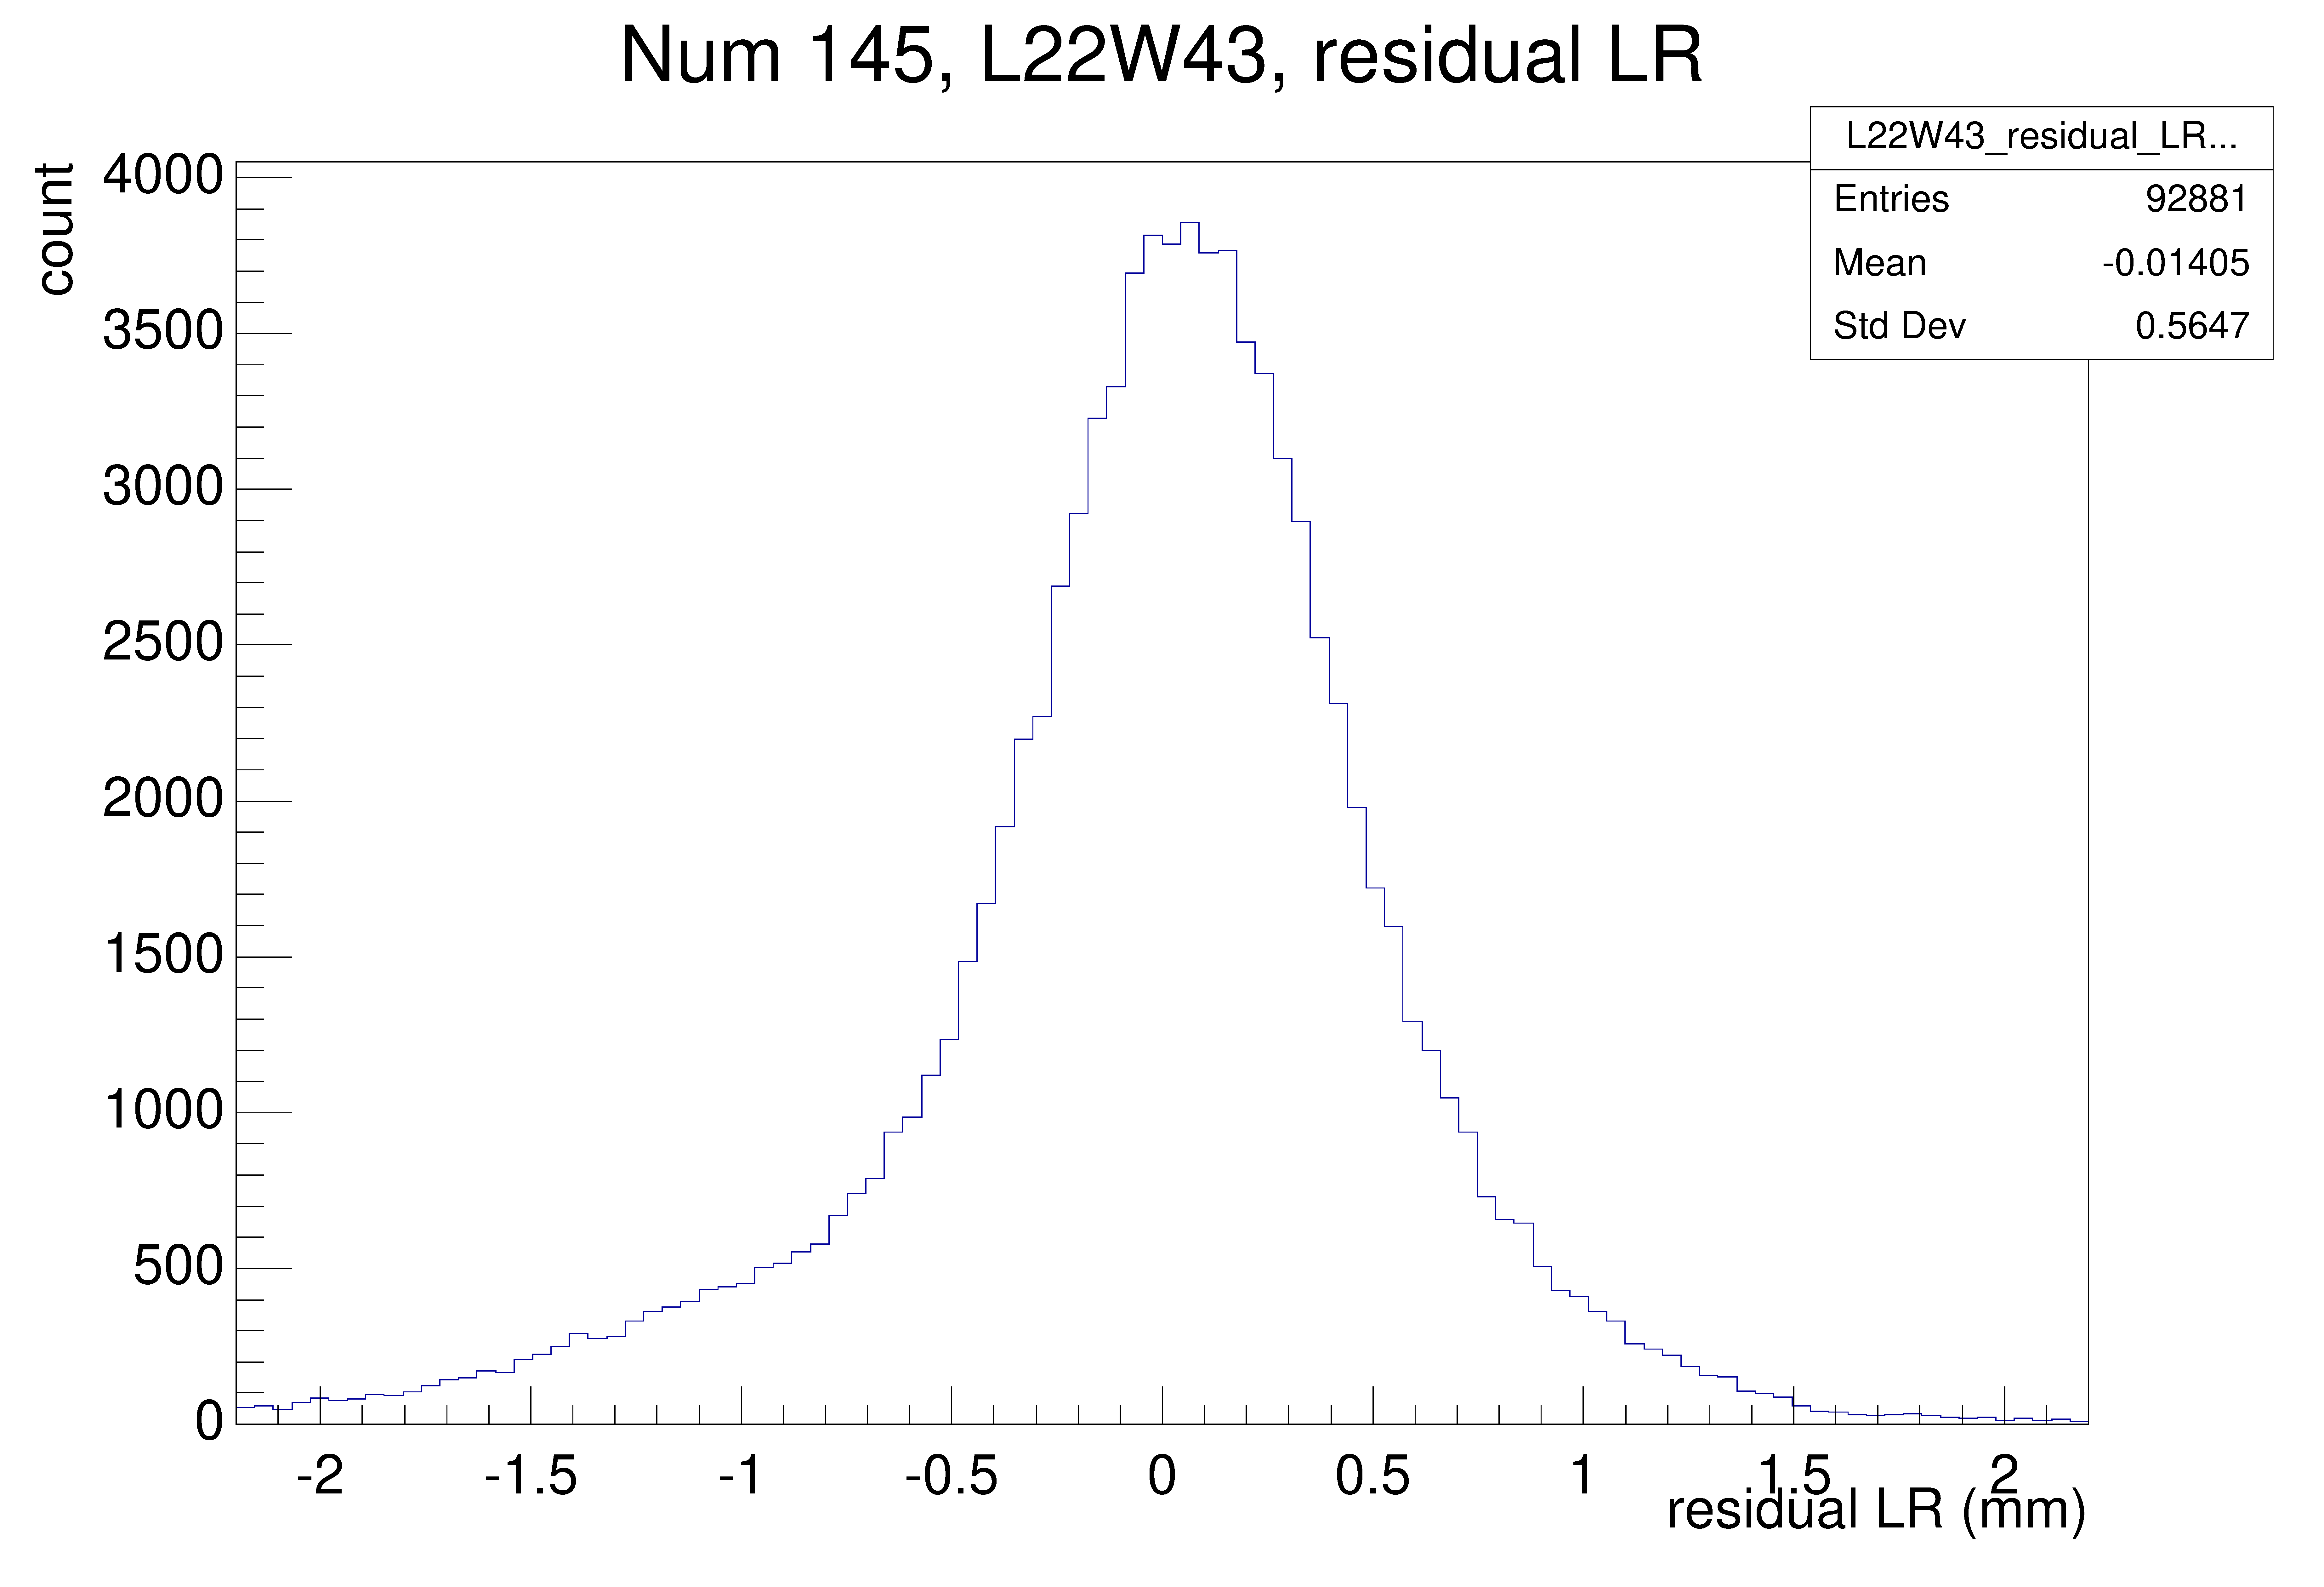
\includegraphics[width=0.20\linewidth]{figures/L22W43_new_tt.pdf} \\
        
        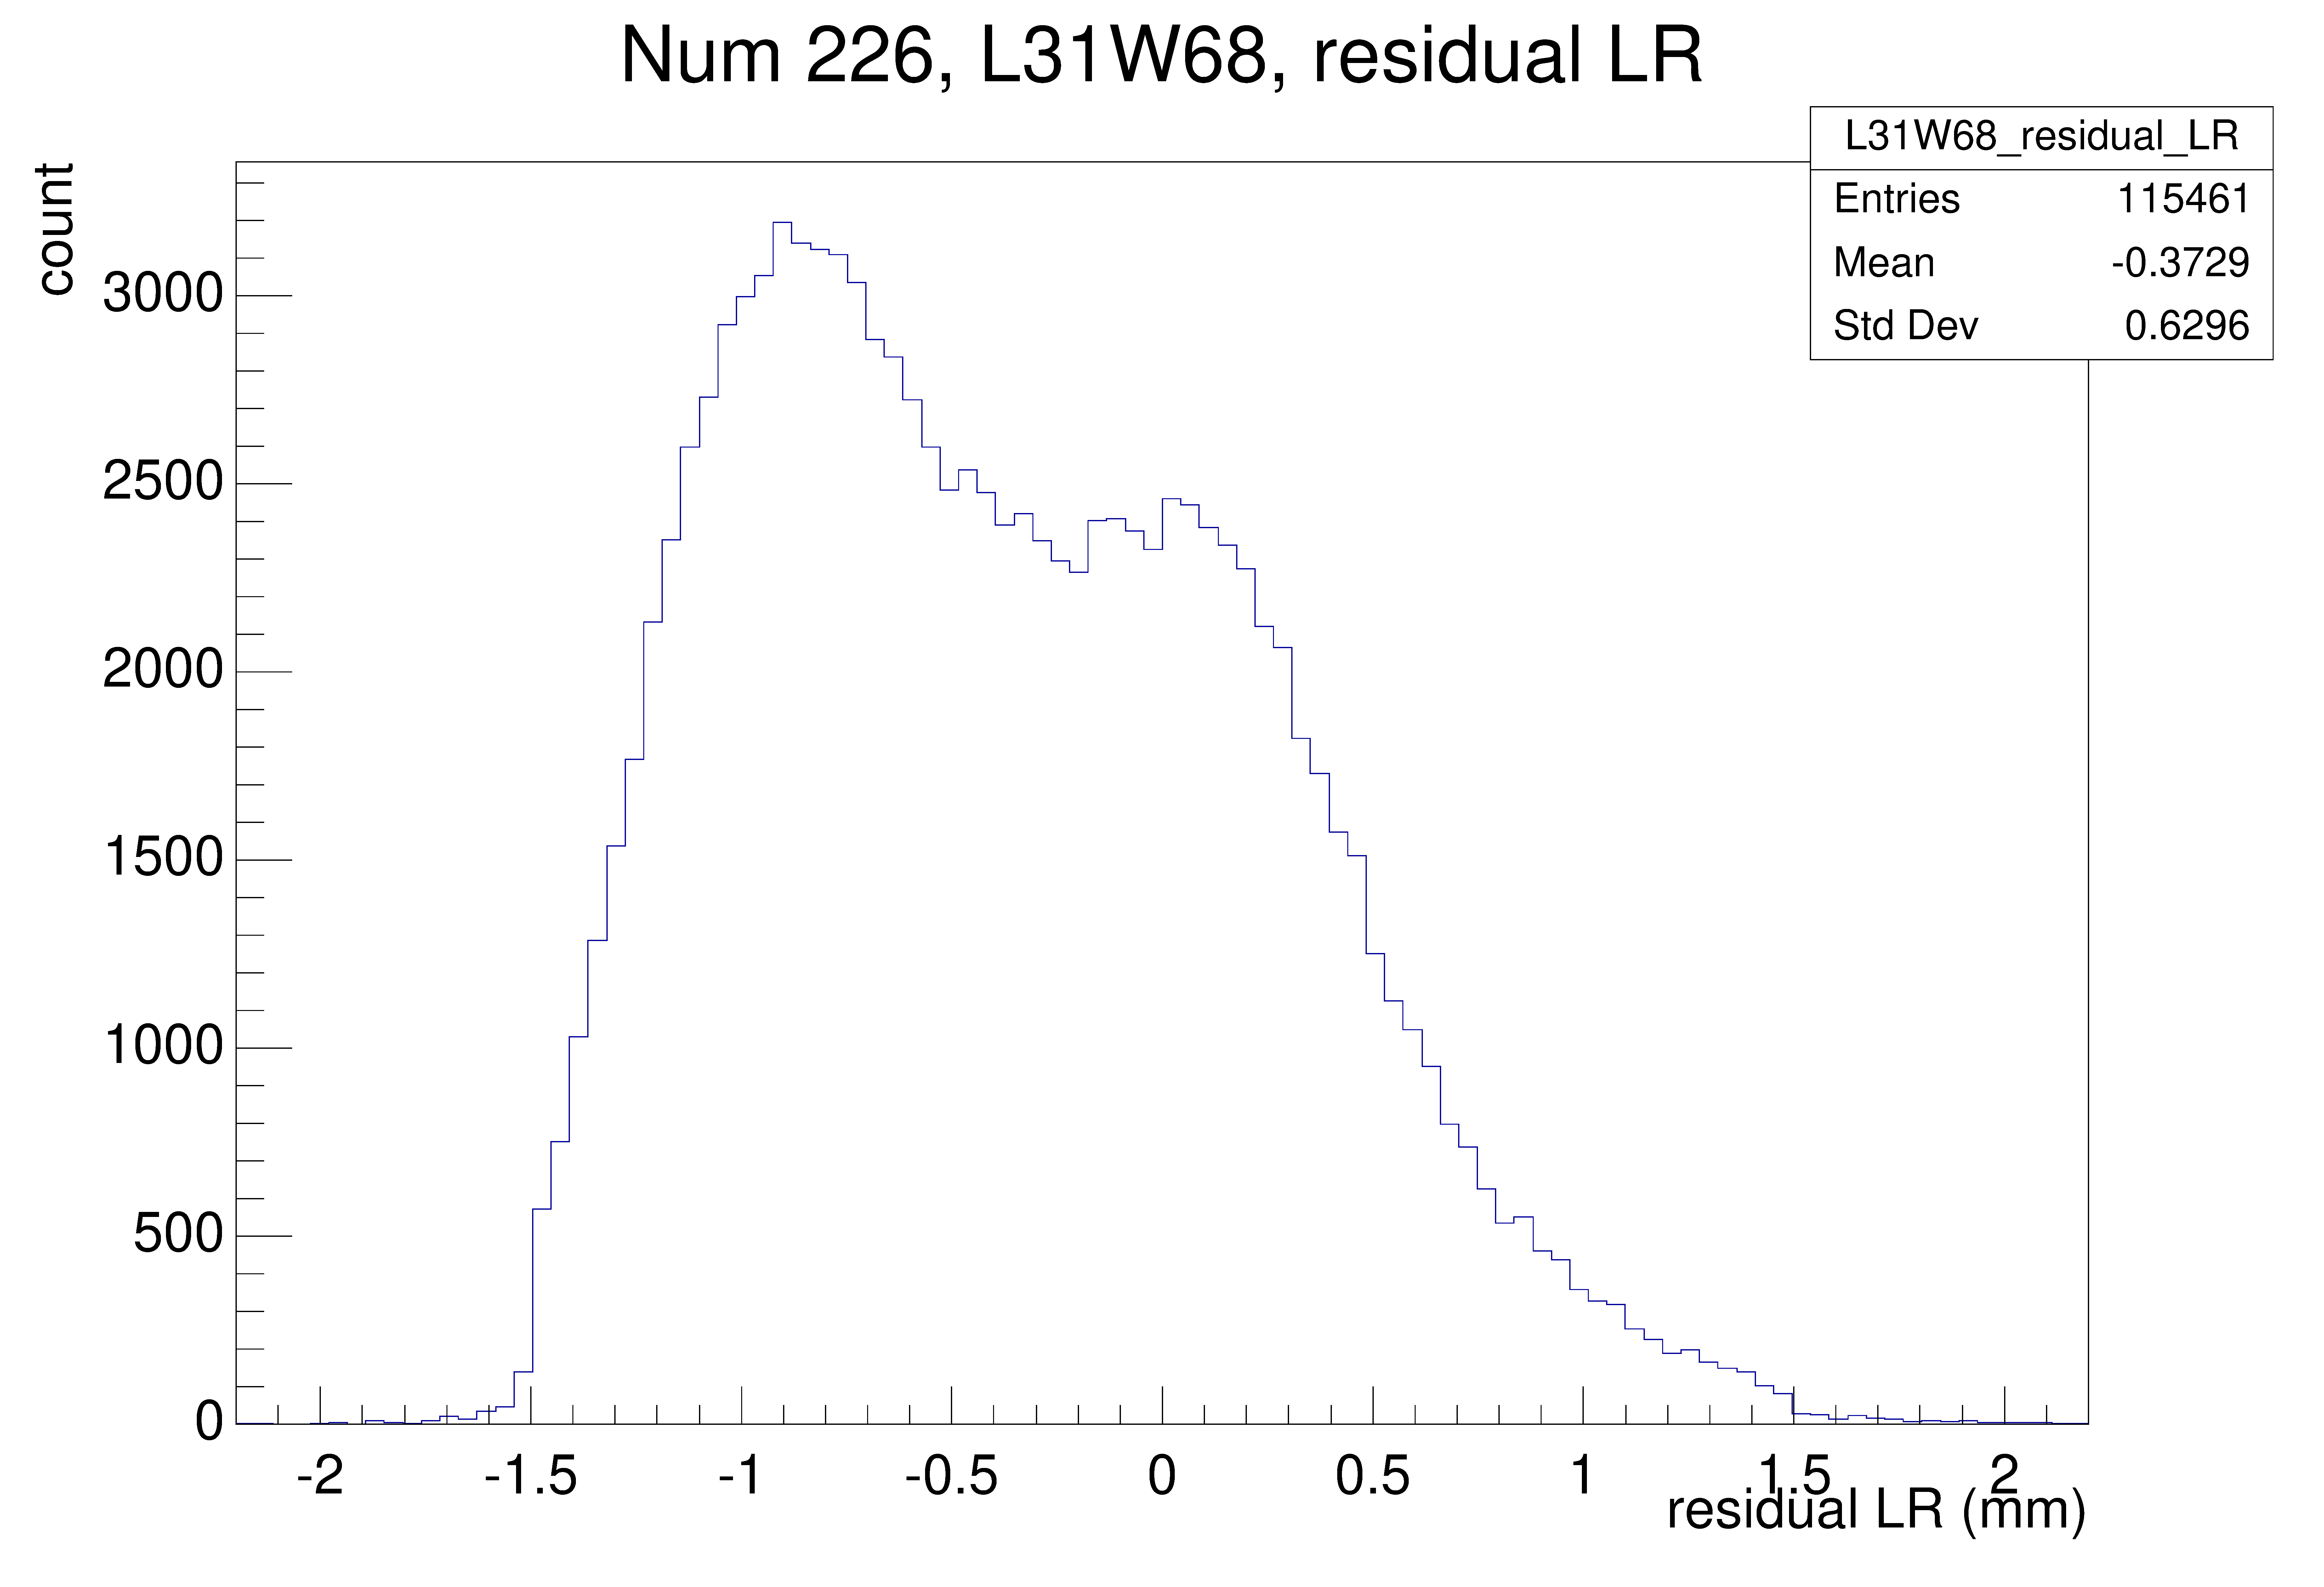
\includegraphics[width=0.20\linewidth]{figures/L31W68_old_tt.pdf} & 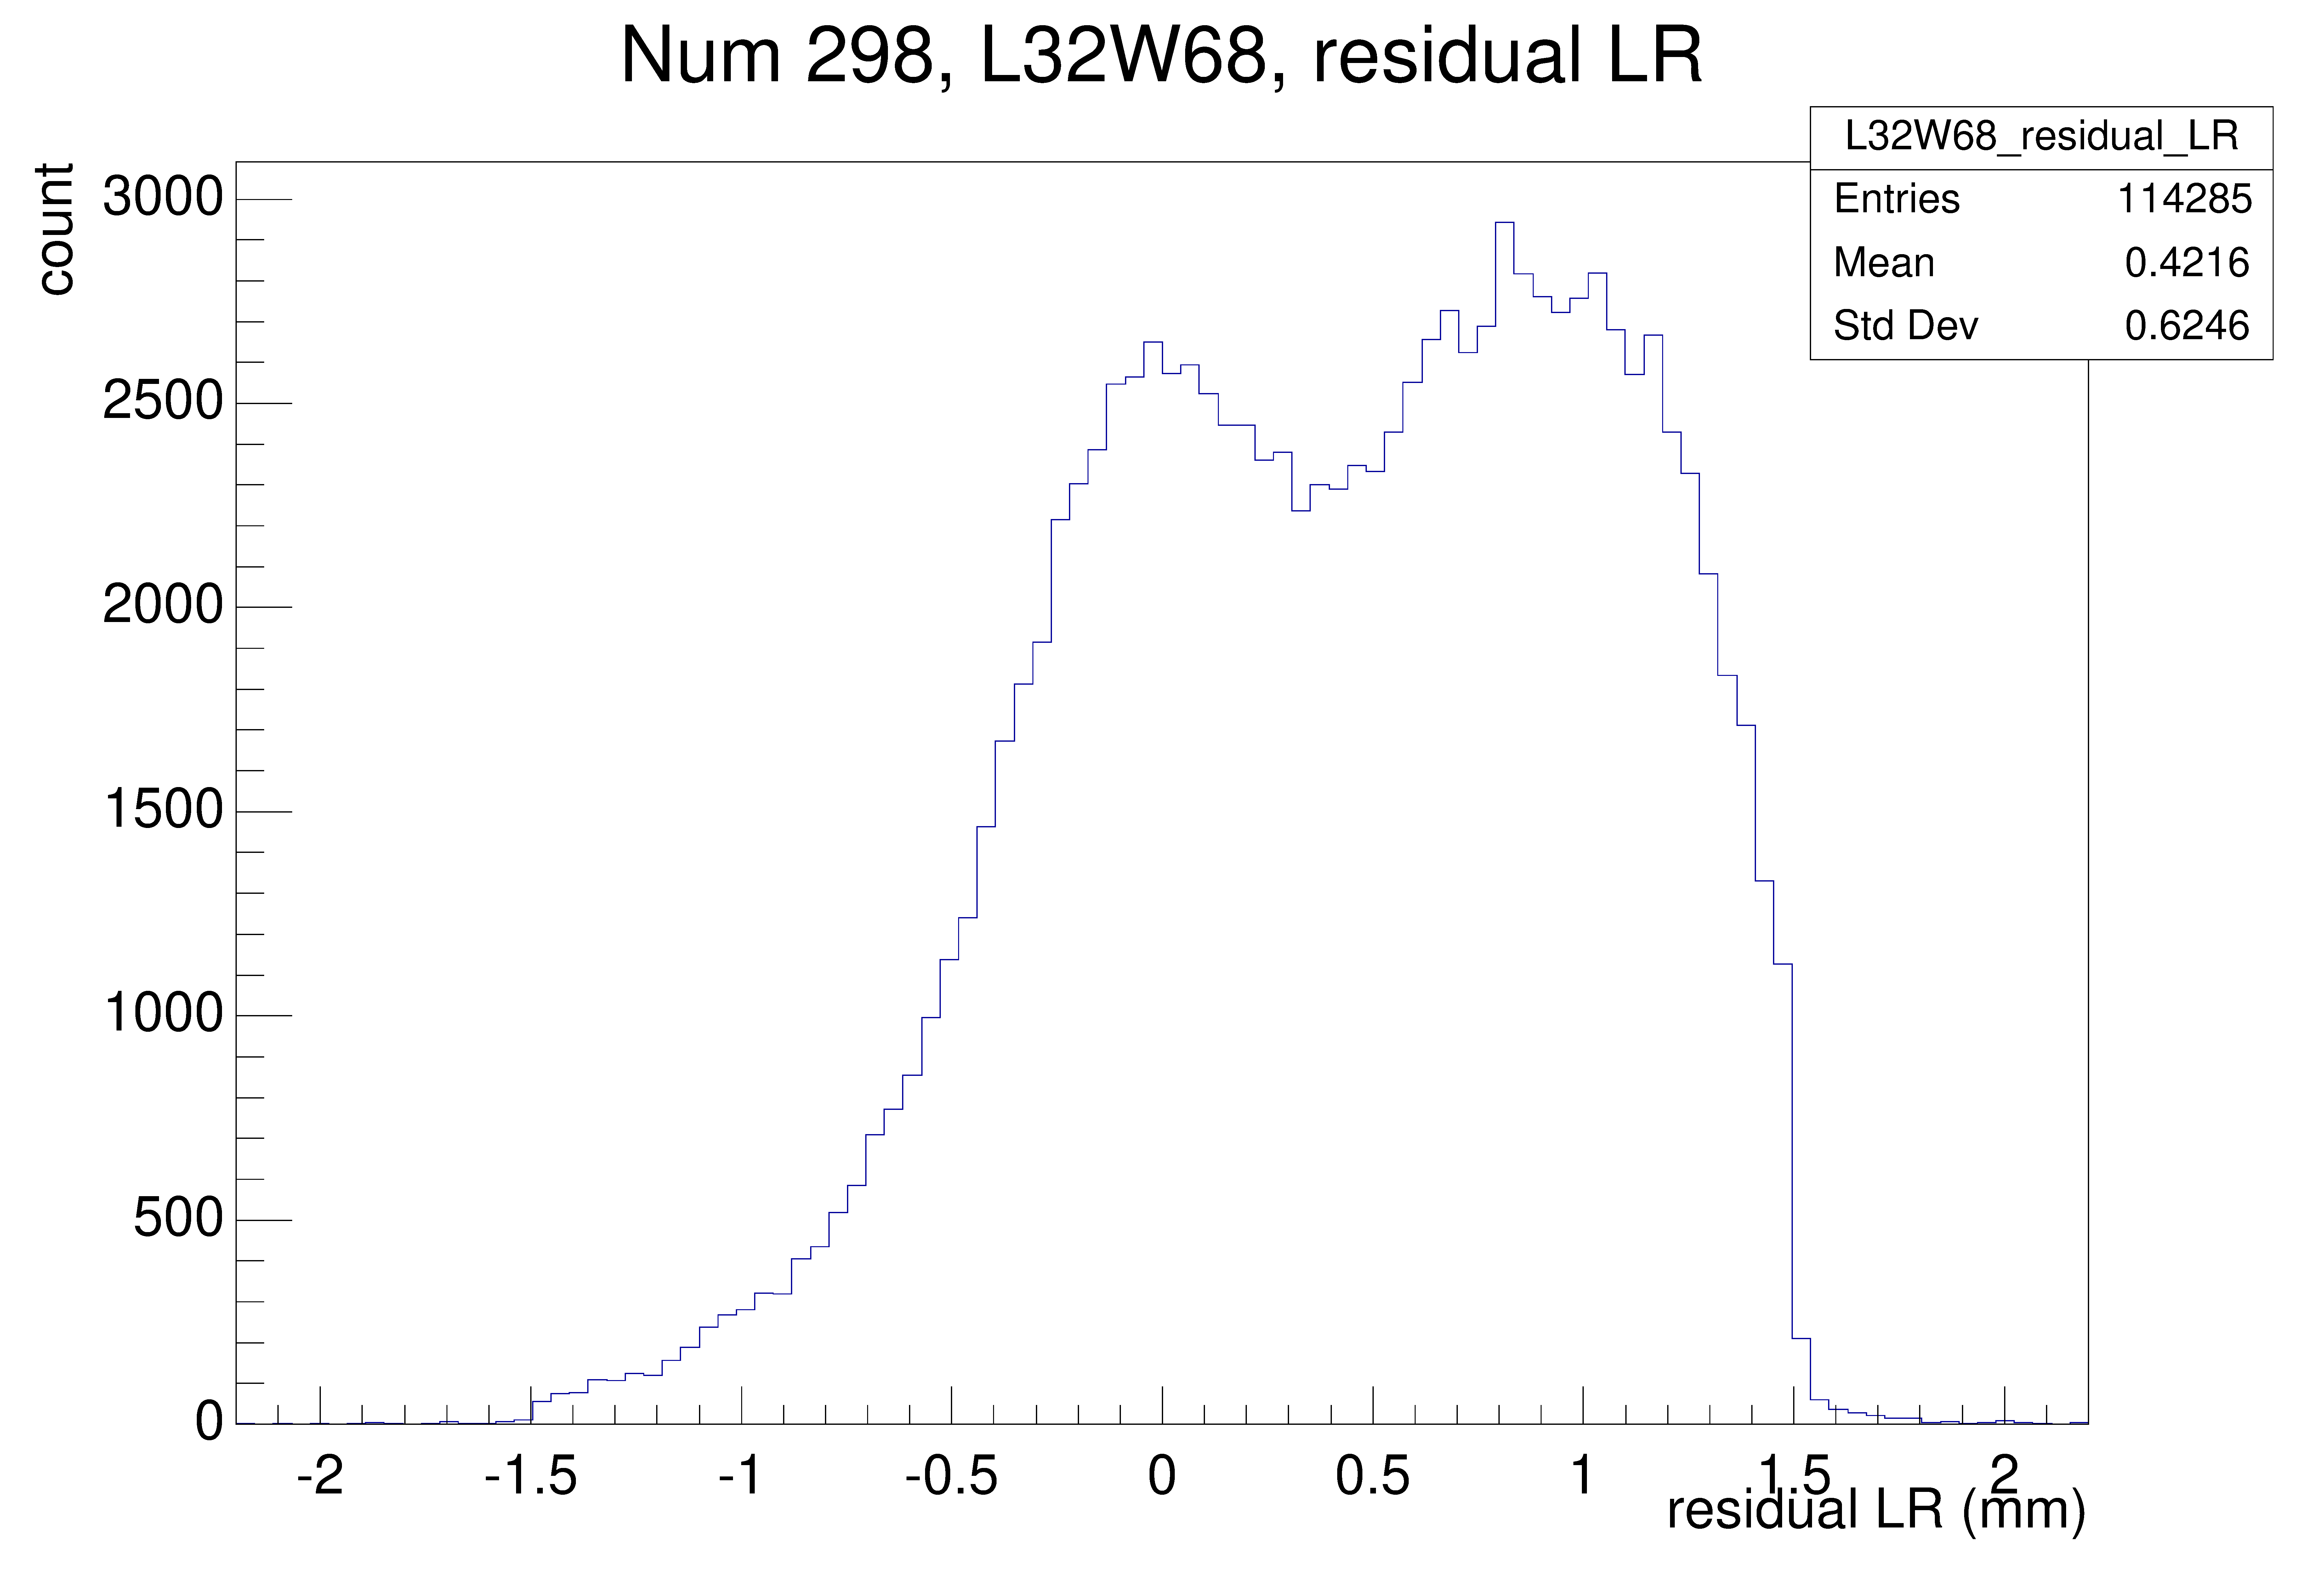
\includegraphics[width=0.20\linewidth]{figures/L32W68_old_tt.pdf} & 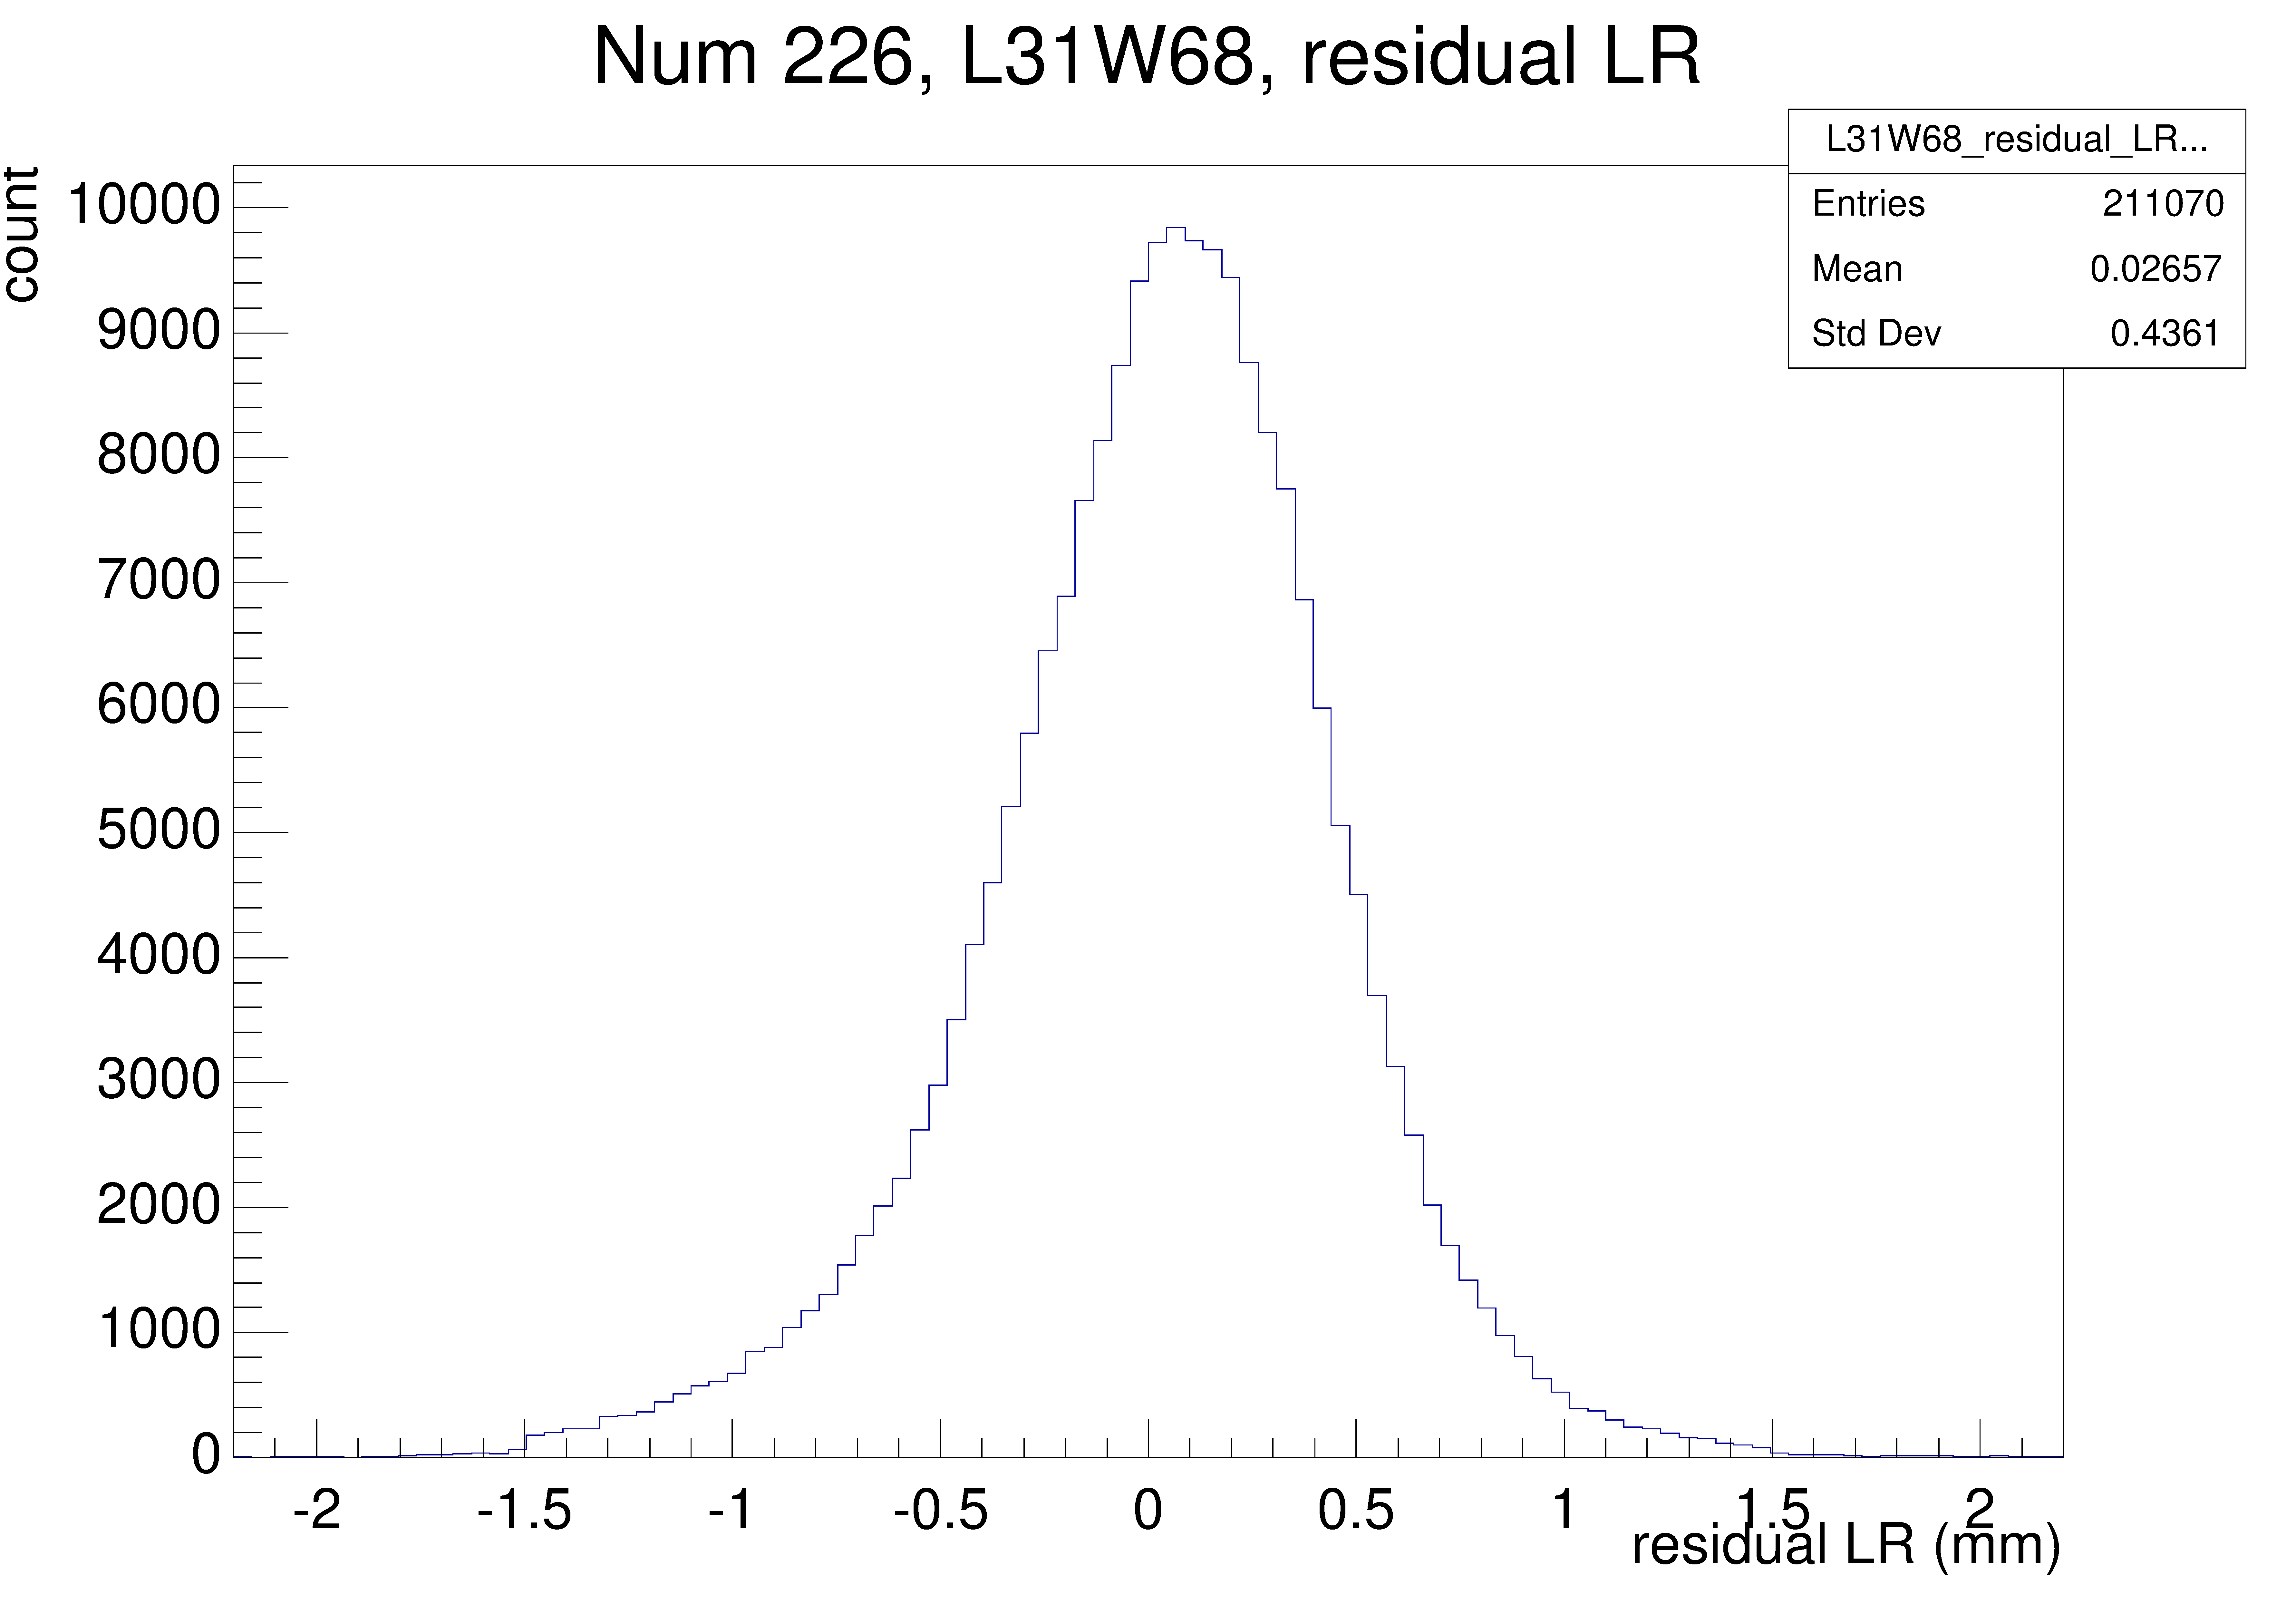
\includegraphics[width=0.20\linewidth]{figures/L31W68_new_tt.pdf} & 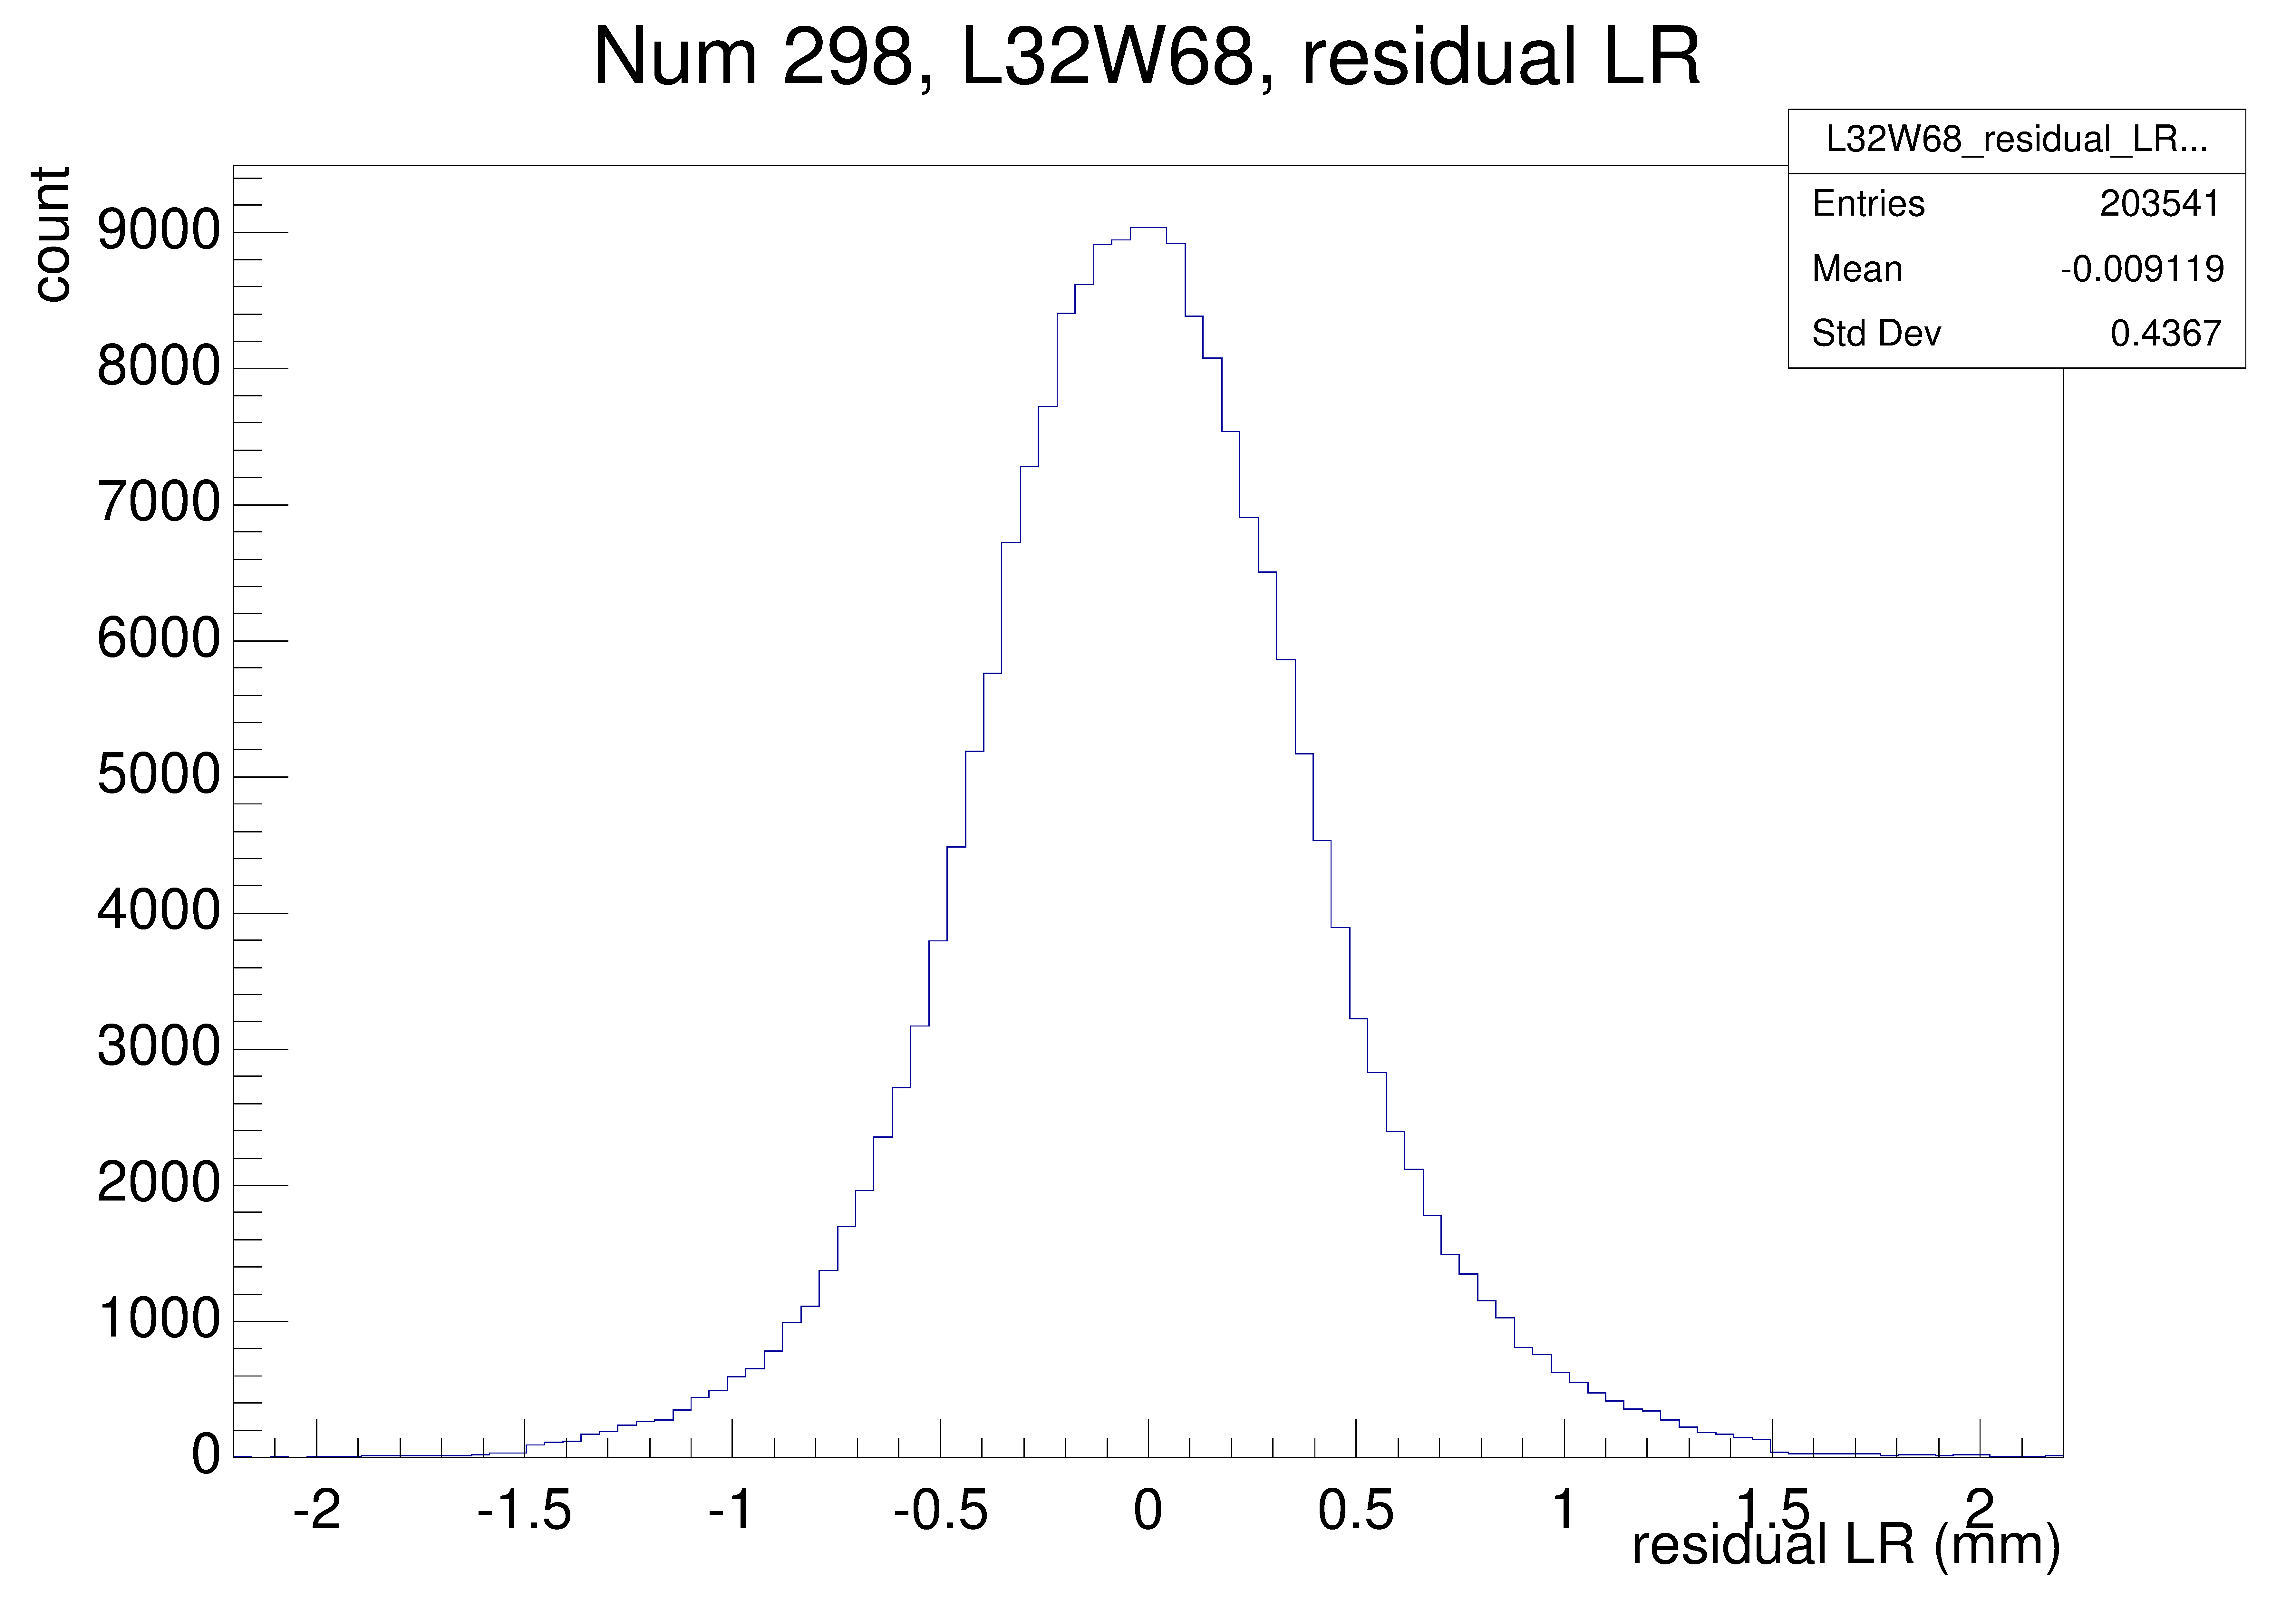
\includegraphics[width=0.20\linewidth]{figures/L32W68_new_tt.pdf} \\
    \end{tabular}

    {\tiny Compared to the other swaps, L31W68 and L32W68 had a peak at 0. Same SL, $\neq$ L, same W  $\rightarrow$ effect difficult to see in Wire versus Phi}

\end{frame}

\begin{frame}{Results - wire swaps}
    \begin{itemize}
        \item Illustration :  Others residual distributions had a bad shape, but they all had a bad $t_0$
    \end{itemize}

    \centering
    \vspace{0.2cm}

    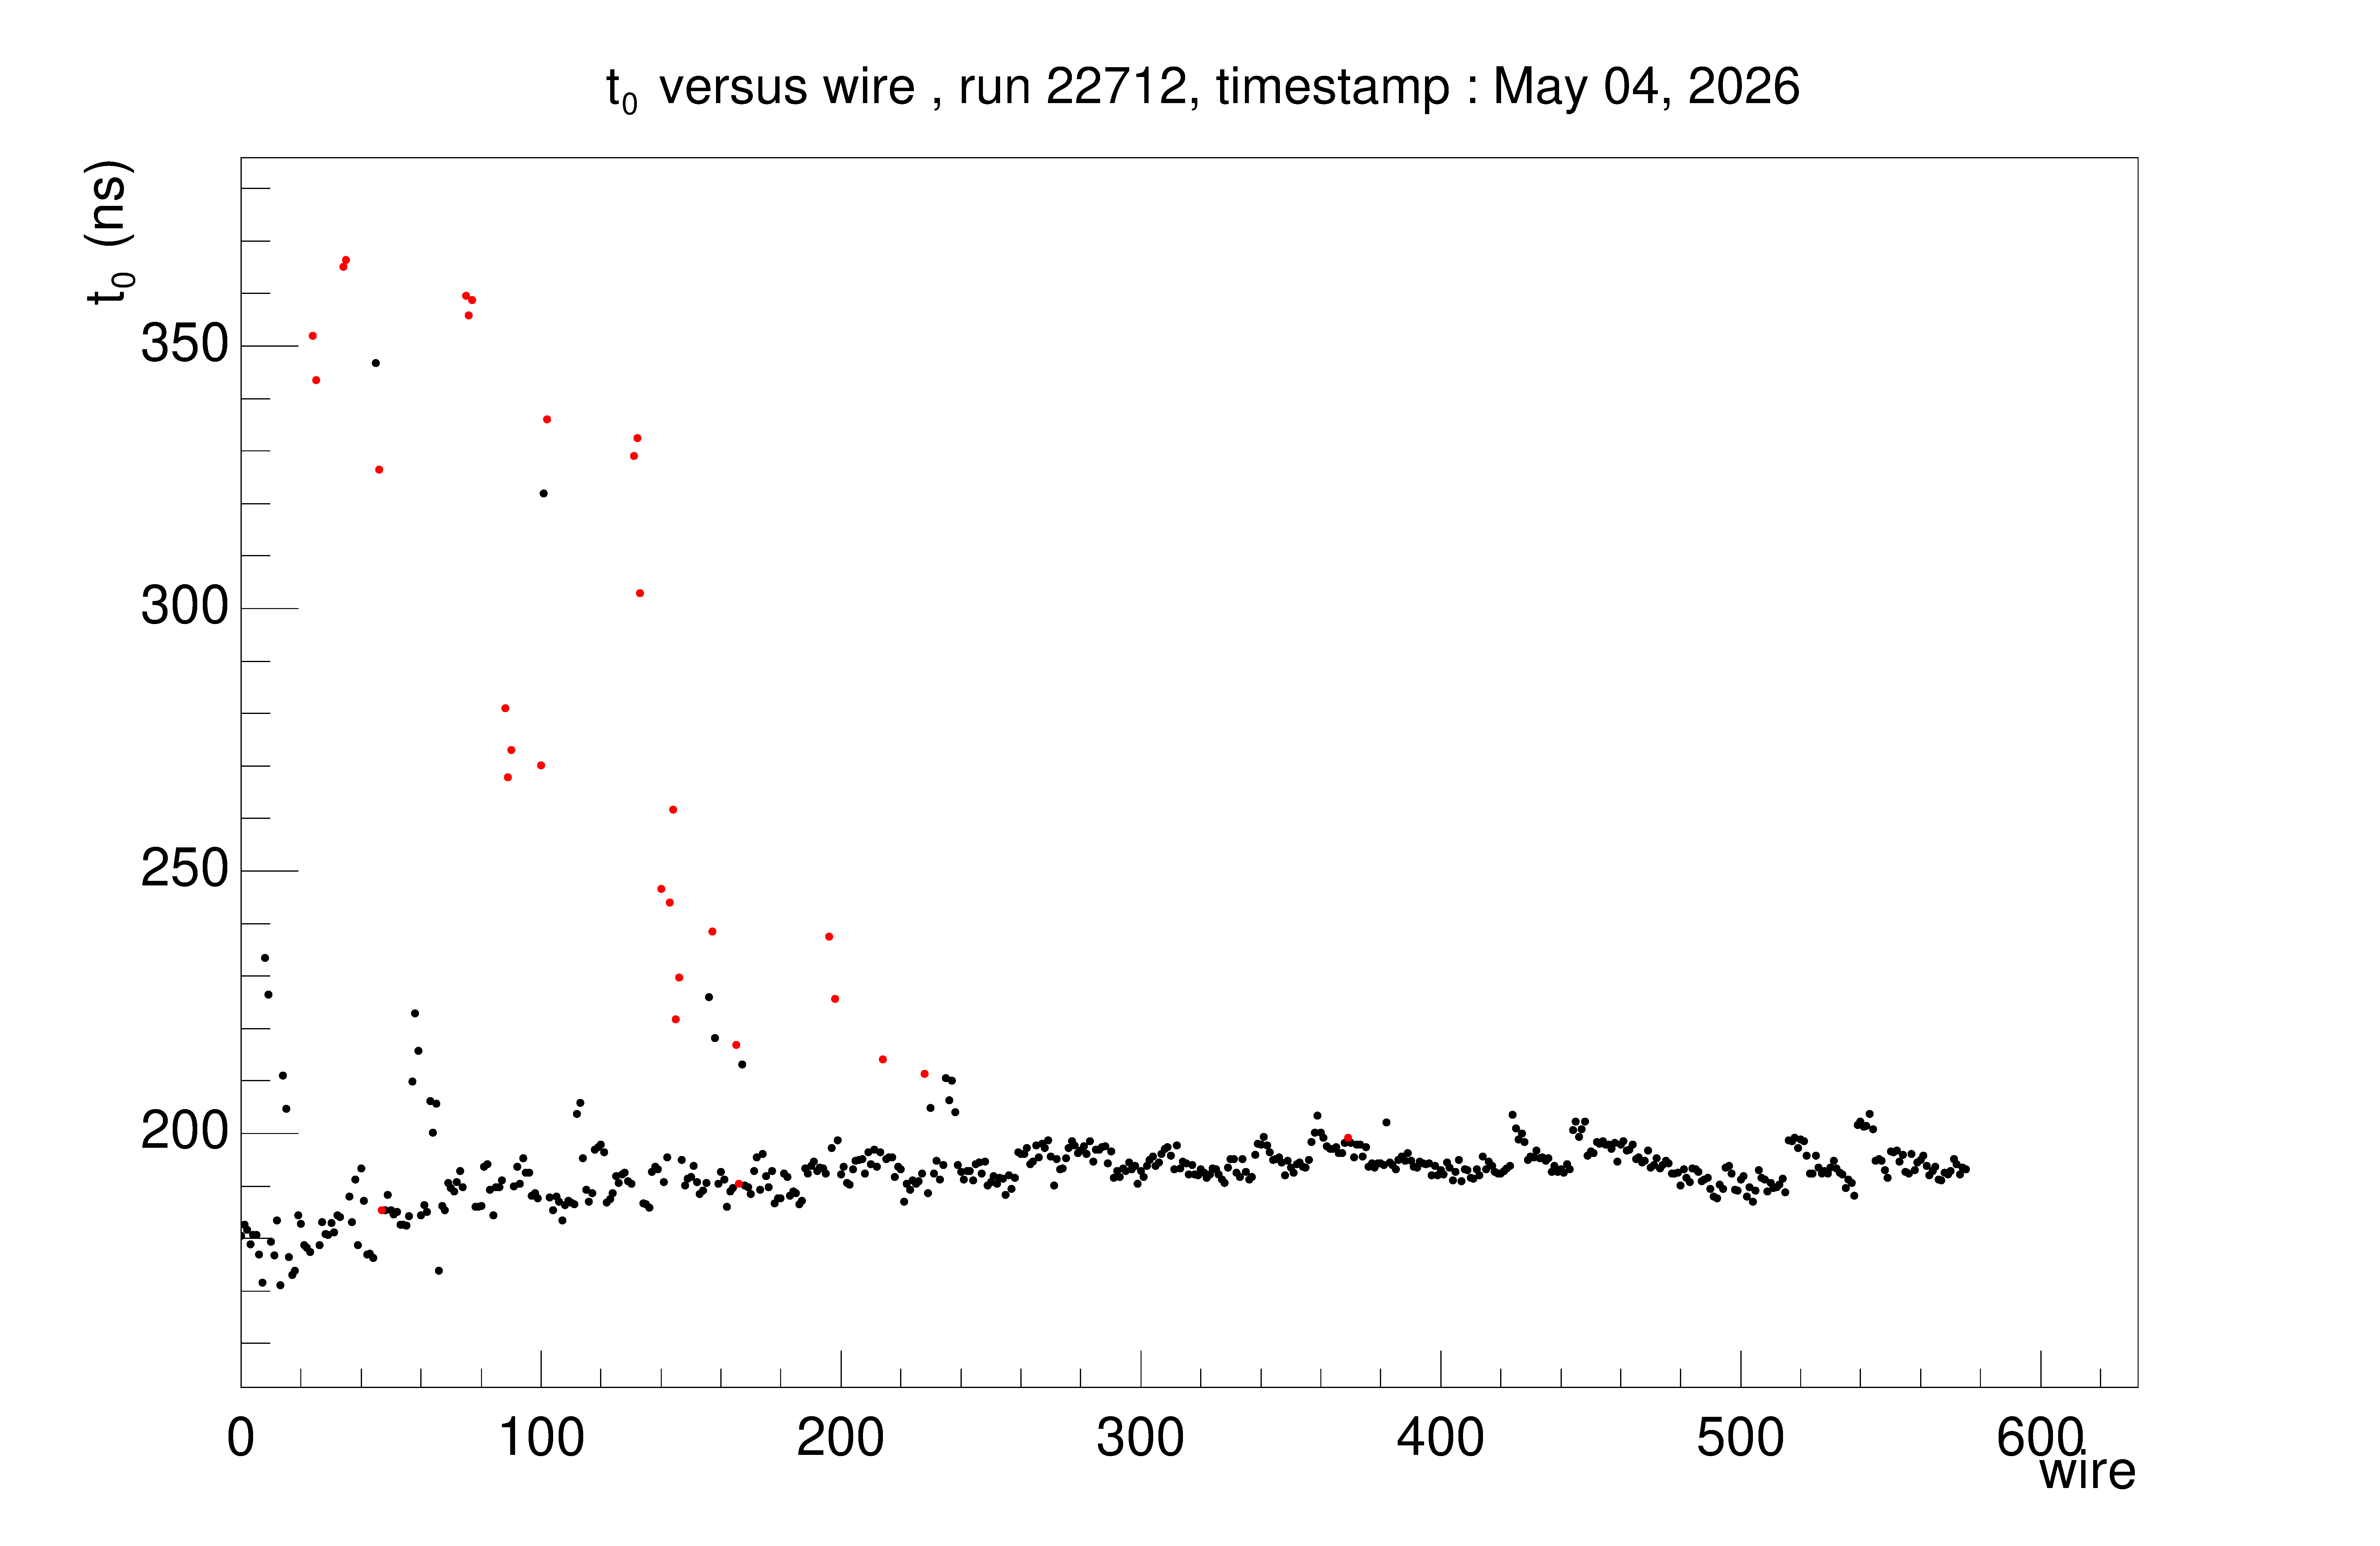
\includegraphics[width=0.8\linewidth]{figures/bad_wires_vs_t0.pdf}

\end{frame}

\begin{frame}{Results - wire swaps}
    \begin{itemize}
        \item Next steps
            \begin{itemize}
                \item Update the translation table with the identified swaps
                \item Update the $t_0$ ?
            \end{itemize}
    \end{itemize}

    \centering
    \vspace{0.2cm}

\end{frame}



% \begin{frame}{Backup slides}
%     \begin{itemize}
%         \item Procedure:
%             \begin{enumerate}
%                 \item We looked at elastic events : electron + track (here: collection of hits only)
%                 \item We computed the theoretical momentum vector of the track $\vec{p}$
%                 \item We made the propagation without doing any fit (i.e no KF correction)
%                 \item We looked at {\color{blue} residual\_LR} (left-right) $\longrightarrow$ sensitive to the alignment
%             \end{enumerate}
%     \end{itemize}
    

%     \vspace{0.2cm}
%     \centering
%     \begin{minipage}{0.42\textwidth}
%         \includegraphics[width=\linewidth]{figures/build/illustration_residual_type.pdf}
%     \end{minipage}

% \end{frame}






\end{document}


